\documentclass[letterpaper,12pt]{article}

% @@@@@@@@@@@@@@@@@@@@@@@@@@@@@@@@@@@@@@@@@@@@@@@@@@@@@@@@@@@@>
% VALORES A MODIFICAR POR USTED:
% @@@@@@@@@@@@@@@@@@@@@@@@@@@@@@@@@@@@@@@@@@@@@@@@@@@@@@@@@@@@>

\usepackage{biblatex}
\addbibresource{bibliografia.bib}

% NOTE: Leer nota en el README sobre la font.

\newcommand{\titulo}{Implementación en AMD ROCm de una simulación computacional del método de Lattice Boltzmann}
\newcommand{\ciudad}{Valparaiso} % e.g. Valparaíso
% TODO: Consultar el formato de los nombres:
\newcommand{\nombrealumno}{Gonzalo Andrés Oberreuter Álvarez}
\newcommand{\nombreprofesor}{Claudio Torres, Ph.D.}
\newcommand{\nombrecorreferente}{Álvaro Salinas, M.Sc.}
% Mes y año del examen
\newcommand{\mesexamen}{Agosto}
\newcommand{\anioexamen}{2021}
% Dedicatoria y agradecimientos
%\newcommand{\dedicatoria}{
%Considerando lo importancia de este trabajo para los alumnos, este apartado es para que el autor entregue palabras personales para dedicar este documento. La extensión puede ser de máximo una hoja y se deben mantener este formato, tipo y tamaño de letra.
%}
\newcommand{\agradecimientos}{
En este momento cúlmine de mi carrera universitaria, quisiera agradecer
\begin{itemize}
    \item A mis padres, por nunca dudar sobre mis habilidades y por el apoyo que siempre me brindaron
    \item A cada compañer@ de carrera que conocí, por haber formado parte de mi vida diaria y, en perspectiva, formar parte de la persona que soy hoy en día 
    \item A los integrantes de la OEUTFSM, por demostrar que estuve equivocado al pensar que después de enseñanza media nunca más tocaría violín, y enriquecer de manera inigualable mis años de universidad, abriendo puertas a eventos que nunca pensé que sucederían
\end{itemize}
finalmente, quisiera agradecer personalmente a Mauricio Barrios por facilitar el uso de su computadora para la experimentación de esta memoria.
}

% @@@@@@@@@@@@@@@@@@@@@@@@@@@@@@@@@@@@@@@@@@@@@@@@@@@@@@@@@@@@>

% Paquete para importar imágenes
\usepackage{graphicx}

% Idioma y fuentes
\usepackage[spanish,es-ucroman]{babel}
\usepackage[T1]{fontenc}
\usepackage{fontspec}
\usepackage{algorithm}
\usepackage{algpseudocode}
\usepackage{amsfonts}

\usepackage{multirow}


%\floatname{algorithm}{Algoritmo}

% Paquete para definir cualquier tamaño de font
\usepackage{anyfontsize}

% Settear font
\setmainfont{Carlito}

\usepackage[letterpaper,top=2.5cm,bottom=3cm,left=3cm,right=3cm,marginparwidth=1.75cm]{geometry}

% Determinar interlineado:
\renewcommand{\baselinestretch}{1.0}

% Eliminar sangrías:
\setlength{\parindent}{0cm}

% Paquete para definir los formatos de los títulos
\usepackage[explicit]{titlesec}

\titleformat{name=\section}[block]{\fontsize{16}{24}\selectfont\bfseries}{}{0pt}{#1}
\titleformat{name=\section,numberless}[block]{\fontsize{16}{24}\selectfont\bfseries}{}{0pt}{#1}
\titlespacing*{name=\section}{0pt}{0pt}{0.5cm}
\titlespacing*{name=\section,numberless}{0pt}{0pt}{0.5cm}

% Separación entre parrafos
\setlength{\parskip}{0.4cm}

% Paquetes de utilidad general
\usepackage{amsmath}
\usepackage{graphicx}
\usepackage{float}

\usepackage{listings}
\usepackage[table]{xcolor}
% Formato de las tablas de contenido
% Para obtener el número de la última página
\usepackage{lastpage}

% Para las captions de minipages
\usepackage{caption}
\usepackage{subcaption}

\usepackage{tabularx}

% Header y footer
\usepackage{fancyhdr}
\fancypagestyle{portada}{
    \lhead{}
    \chead{}
    \rhead{}
    \lfoot{}
    \cfoot{\fontsize{10}{12}\selectfont \thepage}
    \rfoot{}
    \renewcommand{\headrulewidth}{0pt}
}
\fancypagestyle{intermedio}{
    \lhead{}
    \chead{\fontsize{10}{12}\selectfont\MakeUppercase{\titulo}}
    \rhead{}
    \lfoot{}
    \cfoot{\fontsize{10}{12}\selectfont Página \textbf{\thepage}\ de \textbf{\pageref{LastPage}}}
    \rfoot{}
    \renewcommand{\headrulewidth}{1pt}
}

\newcommand{\hlabel}{\phantomsection\label}

% Comandos para secciones
\newcommand{\secnumbersection}[1]{
\addtocounter{section}{1}
\section*{CAPÍTULO \thesection \texorpdfstring{\\}\ #1}
\addcontentsline{toc}{section}{CAPÍTULO \thesection : #1}
\setcounter{subsection}{0}
}
\newcommand{\secnumberlesssection}[1]{
\section*{#1}
\phantomsection
\addcontentsline{toc}{section}{#1}
\setcounter{subsection}{0}
}
\lstset{xleftmargin=2.2em,framexleftmargin=2.2em, showstringspaces=false}


\definecolor{dkgreen}{rgb}{0,0.6,0}
\definecolor{gray}{rgb}{0.5,0.5,0.5}
\lstdefinestyle{CudaStyle}{ 
  language=C++,                % the language of the code
  numberfirstline=true,
  numbersep=5pt,                  % how far the line-numbers are from the code
  backgroundcolor=\color{white},      % choose the background color. You must add \usepackage{color}
  rulecolor=\color{black},        % if not set, the frame-color may be changed on line-breaks within not-black text 
  tabsize=2,                      % sets default tabsize to 2 spaces
  breaklines=true,                % sets automatic line breaking
  breakatwhitespace=false,        % sets if automatic breaks should only 
  keywordstyle=\color{blue},          % keyword style
  commentstyle=\color{gray},       % comment style
  stringstyle=\color{dkgreen},         % string literal style
  escapeinside={\%*}{*)},            % if you want to add LaTeX within your code
  morekeywords={cudaMemcpy, cudaMalloc, cudaFree}
}

% Nombres
\addto\captionsspanish{\renewcommand{\contentsname}{ÍNDICE DE CONTENIDOS}}
\addto\captionsspanish{\renewcommand{\listfigurename}{ÍNDICE DE FIGURAS}}
\addto\captionsspanish{\renewcommand{\listtablename}{ÍNDICE DE TABLAS}}
\makeatletter
\renewenvironment{thebibliography}[1]
     {\secnumberlesssection{REFERENCIAS BIBLIOGRÁFICAS}
      \@mkboth{\MakeUppercase\bibname}{\MakeUppercase\bibname}%
      \list{\@biblabel{\@arabic\c@enumiv}}%
           {\settowidth\labelwidth{\@biblabel{#1}}%
            \leftmargin\labelwidth
            \advance\leftmargin\labelsep
            \@openbib@code
            \usecounter{enumiv}%
            \let\p@enumiv\@empty\@
            \renewcommand\theenumiv{\@arabic\c@enumiv}}%
      \sloppy
      \clubpenalty4000
      \@clubpenalty\clubpenalty\@
      \widowpenalty4000%
      \sfcode`\.\@m}
     {\def\@noitemerr\@
       {\@latex@warning{Empty `thebibliography' environment}}%
      \endlist}
\makeatother

% Personalizar Tabla de Contenidos

\usepackage{tocloft}
\renewcommand{\cftsecfont}{\fontsize{12}{14}\selectfont\fontspec{Carlito}}
\renewcommand{\cftsubsecfont}{\fontsize{12}{14}\selectfont\fontspec{Carlito}}
\renewcommand{\cftsubsubsecfont}{\fontsize{12}{14}\selectfont\fontspec{Carlito}}

\renewcommand\cftfigfont{\fontsize{12}{14}\selectfont\fontspec{Carlito}}

% Links sin color
\usepackage{hyperref}
\hypersetup{
    colorlinks=false,
}

% @@@@@@@@@@@@@@@@@@@@@@@@@@@@@@@@@@@@@@@@@@@@@@@@@@@@@@@@@@@@>
\begin{document}
\sloppy % Para evitar que referencias se escapen de los márgenes.

\pagestyle{portada}
\pagenumbering{roman}
% NOTE: Este archivo contiene la portada, la dedicatoria, los agradecimientos y el resumen.
% __NO ES NECESARIO MODIFICAR ESTE ARCHIVO__, esas se modifican con los comandos que aparecen en main.tex
%@@@@@@@@@@@@@@@@@@@@@@@@@@@@@@@@@@@@@@@@@@@@@@@@@@@@@@@@@@@@@@
\begin{titlepage}
\begin{center}
\noindent
{\fontsize{18}{22}\selectfont UNIVERSIDAD TÉCNICA FEDERICO SANTA MARÍA \\}
{\fontsize{16}{19}\selectfont DEPARTAMENTO DE INFORMÁTICA \\}
{\fontsize{16}{19}\selectfont \MakeUppercase{\ciudad}\ - CHILE \\}
\vspace{1.5cm}

\includegraphics[width=4.41cm,height=3.34cm]{Logo/logo.jpg} \\
\vspace{1.5cm}
{\fontsize{20}{24}\selectfont ``\MakeUppercase{\titulo}'' \\}
\vfill
{\fontsize{16}{19}\selectfont \MakeUppercase{\nombrealumno} \\}
\vfill
{\fontsize{16}{19}\selectfont MEMORIA PARA OPTAR AL TÍTULO DE \\}
{\fontsize{16}{19}\selectfont INGENIERO CIVIL EN INFORMÁTICA \\}
\vspace{1.5cm}
{\fontsize{14}{17}\selectfont Profesor Guía: \nombreprofesor \\}
{\fontsize{14}{17}\selectfont Profesor Correferente: \nombrecorreferente \\}
\vspace{2.5cm}
{\fontsize{14}{17}\selectfont \mesexamen\ - \anioexamen \\}
\end{center}
\end{titlepage}

%@@@@@@@@@@@@@@@@@@@@@@@@@@@@@@@@@@@@@@@@@@@@@@@@@@@@@@@@@@@@@@
\iffalse
\newpage

\
\vfill
\vfill
\begin{flushright}
\noindent {\fontsize{16}{19}\selectfont \textbf{DEDICATORIA} \\}
\end{flushright}
\begin{flushright}
\noindent \dedicatoria
\end{flushright}
\vfill
\fi
%@@@@@@@@@@@@@@@@@@@@@@@@@@@@@@@@@@@@@@@@@@@@@@@@@@@@@@@@@@@@@@
\newpage
\setcounter{page}{2}
\begin{center}
\noindent {\fontsize{16}{19}\selectfont \textbf{AGRADECIMIENTOS} \\}
\end{center}
\noindent \agradecimientos
\vfill
%@@@@@@@@@@@@@@@@@@@@@@@@@@@@@@@@@@@@@@@@@@@@@@@@@@@@@@@@@@@@@@
\newpage
\secnumberlesssection{RESUMEN}
\vspace{0.3cm}
\noindent La computación paralela de alto rendimiento en GPUs, es una tecnología a la vanguardia para la resolución de problemas complejos de la ciencia de la computación.
De aquellas tecnologías de HPC que se generan, ROCm se plantea como una alternativa para la programación y ejecución de software en GPUs de AMD.
Con esto, se desarrollarán diferentes experimentaciones de programación de propósito general en GPU para hacer una comparativa en torno al rendimiento entre el uso de tarjetas AMD y NVIDIA.
La experimentación culminará con la ejecución de una implementación del Método de Lattice Boltzmann con condiciones de borde abiertas para la resolución de las ecuaciones de agua poco profunda, con tal de concluir respecto a los resultados, expresar la utilidad real de ROCm y comentar respecto a su uso en general. \ \\
\vspace{0.3cm} \\
\noindent \textbf{Palabras Clave}: Método de Lattice Boltzmann, AMD ROCm, NVIDIA CUDA, Computación de Alto Rendimiento  \ \\
% @@@@@
\vspace{1.2cm} \\
% @@@@@
%\noindent {\fontsize{16}{19}\selectfont \textbf{ABSTRACT}}
%\vspace{1.2cm} \\
\secnumberlesssection{ABSTRACT}
\vspace{0.3cm}
\noindent High performance computing in GPUs, is a vanguard technology for the resolution of complex problems in computer science. 
From those HPC technology that are being generated, ROCm is proposed as an alternative for the programming and execution of software in AMD's GPUs.
With this, different general purpose GPU programming experiments will be developed so a comparative of the performance of AMD and NVIDIA GPUs can be done.
The experimentation will culminate with the execution of an implementation of the Lattice Boltzmann Method with open boundary conditions for the resolution of the shallow water equations, in order to conclude about the results, express the real utility of ROCm and comment its general usage. \ \\
\vspace{0.3cm} \\
\noindent \textbf{\emph{Keywords}}: Lattice Boltzmann Method, AMD ROCm, NVIDIA CUDA, High Performance Computing \ \\
%@@@@@@@@@@@@@@@@@@@@@@@@@@@@@@@@@@@@@@@@@@@@@@@@@@@@@@@@@@@@@@


%\newpage
%\secnumberlesssection{GLOSARIO}

Aquí se deben colocar las siglas mencionadas en el trabajo y su explicación, por orden alfabético. Por ejemplo: \\

{\setlength{\parskip}{0cm} % Para evitar saltar entre cada elemento nombrado.
%Colocar aquí siglas:
DI: Departamento de Informática.

UTFSM: Universidad Técnica Federico Santa María.
}


%Índice de contenidos:
\newpage
\thispagestyle{portada}
\tableofcontents

%Índice de figuras:
\newpage
\thispagestyle{portada}
\phantomsection
\addcontentsline{toc}{section}{ÍNDICE DE FIGURAS}
\listoffigures
\phantomsection
\addcontentsline{toc}{section}{ÍNDICE DE TABLAS}

\newpage

\listoftables

\newpage

\pagestyle{intermedio}
\pagenumbering{arabic}
\secnumberlesssection{INTRODUCCIÓN}

En los últimos años, términos como \textit{Machine Learning} o \textit{Data Mining} han sido protagónicos en el área de la ciencia de la computación por su aplicabilidad a la hora de abordar problemas complejos.
%por un aumento en su uso/empleo a la hora de resolver problemas complejos.
Sin embargo, el problema de trabajar con estos campos es la dificultad de su escalabilidad, al requerir un gran tamaño de operaciones elementales, lo cual significa que se debe utilizar bibliotecas y hardware especializado para poder abordar estos problemas.
Por otro lado, al tratar de compensar esto último es que se ha aplicado la Computación de Alto Rendimiento (del inglés, High Performance Computing), que cual consiste en el uso de clústeres de nodos computacionales, supercomputadores o programación paralela para la solución de aquellos problemas de ingeniería, ciencia o gestión que necesitan de un alto rendimiento.

Debido al avance de la tecnología y con tal de beneficiar el uso de la Computación de Alto Desempeño es que desde el inicio de la década se ha empezado a utilizar el potencial computacional de Unidades de Procesamiento Gráfica (del inglés, Graphic Processing Unit o GPU) por sobre las Unidades de Procesamiento Central (del inglés, Central Processing Unit o CPU) debido a la arquitectura que poseen. 
En particular, esto es por que una CPU está diseñada para manejar rápidamente una gama amplia de tareas, mientras que una GPU está diseñada originalmente para el renderizado de imágenes y videos en alta resolución \cite{gpu}, lo cual sumado a la gran cantidad de unidades de procesamiento de GPUs, presenta la posibilidad del uso dedicado de estas en programación paralela.
Por esto, es que se ha preferido el uso de GPUs al momento de realizar tareas de alto desempeño, ya que el rendimiento en términos de la cantidad de operaciones de punto flotante por segundo (del ingles, Floating-Point Operation per Second o FLOPs) es mucho mayor en tarjetas de procesamiento gráfico que de procesamiento central, tomando en cuenta componentes con características parecidas.
Esta diferencia en el rendimiento se debe principalmente, a que si bien una GPU posee una velocidad de reloj interno mucho menor al de una CPU, su cantidad de unidades de procesamiento es mucho mayor, generando mejores resultados en aplicaciones a problemas que sacan ventaja de la programación paralela.

Las simulaciones computacionales, corresponden a programas informáticos cuyo fin es poder simular situaciones en base a modelos de distintas áreas de estudio.
Aquellas simulaciones físicas con menos probabilidad de ocurrencia, tales como tsunamis o huracanes, son en las que hay un mayor enfoque pues normalmente son las que más importancia e impacto producen sobre la vida cotidiana.
La simulación de lo anterior, depende además de la forma en que se modele el problema deseado, el tipo de escala que se utilice y las condiciones de borde que se planteen.

En esta memoria, se presentará una implementación de la simulación computacional de tsunamis utilizando ROCm, una plataforma de desarrollo relativamente nueva de la compañía estadounidense de semi conductores AMD~\cite{rocm}, la cual permite la ejecución de código en GPU sobre tarjetas de la misma marca, lo cual permitirá realizar tanto una comparativa entre el rendimiento de los componentes utilizados como la creación instancias de simulaciones de dinámica de fluidos en términos de lo que sería el inicio de un tsunami. 

La estructura de esta memoria es la siguiente; el Capítulo~\hyperref[sec:1]{1} presentará la definición del problema a tratar y una descripción de de las tecnologías a utilizar; el Capítulo~\hyperref[sec:2]{2} hará una revisión general del estado del arte sobre el uso de ROCm en investigaciones; en el Capítulo~\hyperref[sec:3]{3} se explicará la teoría detrás del trabajo realizado; el Capítulo~\hyperref[sec:4]{4} expondrá los resultados de las experimentaciones propuestas y en el Capítulo~\hyperref[sec:5]{5} se harán conclusiones respecto al trabajo realizado.


\newpage
\secnumbersection{Definición del problema} 
\hlabel{sec:1}

Teniendo como contexto el creciente uso de programación en GPUs, es que nace el concepto de GPGPU (del ingles, General-Purpose computing on Graphics Processing Units) y es que se plantea el problema a tratar en esta memoria.
Este concepto consta de un cambio en el rol de las tarjetas gráficas, desde renderizar todo lo relacionado al despliegue gráfico de un computador, al uso de su gran cantidad de recursos de procesamiento en temas más generales.
Por esta razón, es que se han generado una cantidad considerable de plataformas de desarrollo las cuales permiten crear códigos apuntados a ejecutarse en GPUs que aprovechen las características de su arquitectura, sobre todo el uso de computación paralela \cite{gpuev}.

\begin{figure}[h]
    \centering
    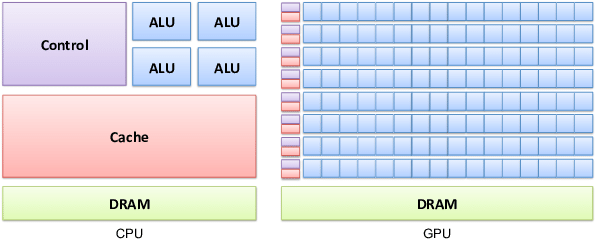
\includegraphics[scale=0.7]{Figures/arch.png}
    \caption{Arquitectura CPU versus GPU, fuente: \cite{arch}.}
    \label{fig:1}
\end{figure}

Las plataformas de desarrollo más actuales tienen como característica una compilación más enfocada en que la ejecución de los binarios esté optimizada a la arquitectura y los núcleos presentes en la GPU que se utilice y que no presente problemas en el paralelismo, como cumplir condiciones de carrera, consistencia en la escritura/lectura, etc.
Actualmente dentro de este tipo de entorno de software, destacan OpenCL, Halide, ROCm y CUDA, sin embargo este último ha tenido una popularidad mayor, al ser desarrollado y distribuido de forma \textit{open-source} por NVIDIA para ser utilizado únicamente por GPUs de la misma compañía.
Debido a esta restricción existente, es que se plantea el uso de ROCm \cite{rocm} para la implementación de esta memoria, ya que es desarrollado por AMD y se plantea como alternativa directa de CUDA y NVIDIA.

Además, dentro de las características favorables del uso de ROCm se encuentra el lenguaje de programación HIP (acrónimo en inglés de Heterogeneous-Computing Interface for Portability), el cual tiene la capacidad computacional de tanto ejecutar código de ROCm en tarjetas gráficas AMD como de traducir código a lenguaje CUDA y ejecutarlo en tarjetas gráficas NVIDIA, gracias a la herramienta Hipify.

\begin{figure}[h]
    \centering
    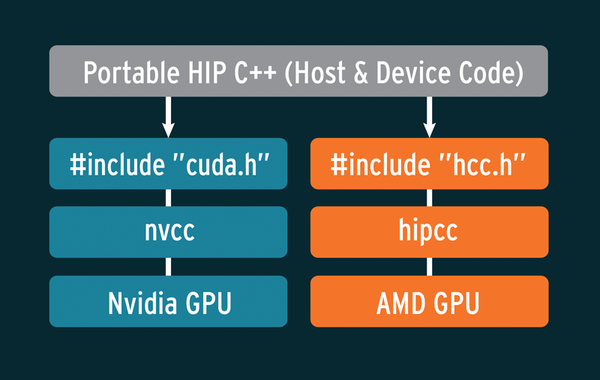
\includegraphics[height=.4\textwidth]{Figures/hipify.png}
    \caption{Diagrama de flujo desde HIP hasta el dispositivo utilizado.}
    \label{fig:2}
\end{figure}

Por otro lado, hasta la última versión lanzada de ROCm, esta tiene soporte para variadas librerías asociadas al uso de HCP, destacando como por ejemplo:

\begin{itemize}
    \item rocBLAS: Conjunto de rutinas asociadas a la ejecución de BLAS (del inglés, Basic Linear Algebra Subprograms), la cual especifica rutinas de bajo nivel sobre operaciones de algebra linear. Este conjunto de software comprende los 3 niveles de operaciones BLAS:
    \begin{itemize}
        \item Nivel 1, sobre operaciones vectoriales en matrices escalonadas, o del tipo 
        \begin{equation*}
            \mathbf{a}\leftarrow \alpha \mathbf{x} + \mathbf{y}
        \end{equation*}
        en donde $\mathbf{a},\mathbf{x},\mathbf{y} \in \mathbb{R}^{n}$ y $\alpha \in \mathbb{R}$.
        \item Nivel 2, sobre operaciones matriz-vector generalizadas (también conocidas como \textit{gemv}), o del tipo
        \begin{equation*}
            \mathbf{a} \leftarrow A\mathbf{x} + \beta \mathbf{y}
        \end{equation*}
        en donde $\mathbf{a},\mathbf{x},\mathbf{y} \in \mathbb{R}^n$, $A \in \mathbb{R}^{n\times n}$ y $\beta \in \mathbb{R}$.
        \item Nivel 3, sobre operaciones matriz-matriz generalizadas (también conocidas como \textit{gemm}), o del tipo
        \begin{equation*}
            A \leftarrow \alpha X\,Y + \beta Z
        \end{equation*}
        en donde $X,Y,Z \in \mathbb{R}^{n\times n}$ y $\alpha,\beta \in \mathbb{R}$.
    \end{itemize}
    \item PyTorch, TensorFlow, Caffe: Librerías asociadas a la construcción, entrenamiento y evaluación de redes neuronales. 
    Estas son útiles al momento de querer entrenar una red neuronal utilizando una gran cantidad de neuronas junto a un gran volumen de datos de entrenamiento, lo cual implicaría un alto costo computacional en caso de desarrollarse de forma secuencial.
    \item rocFFT: Librería de software para computar transformadas rápidas de fourier (del inglés, Fast Fourier Transform), escrita en HIP¨.
\end{itemize}

\begin{figure}[ht]
    \centering
    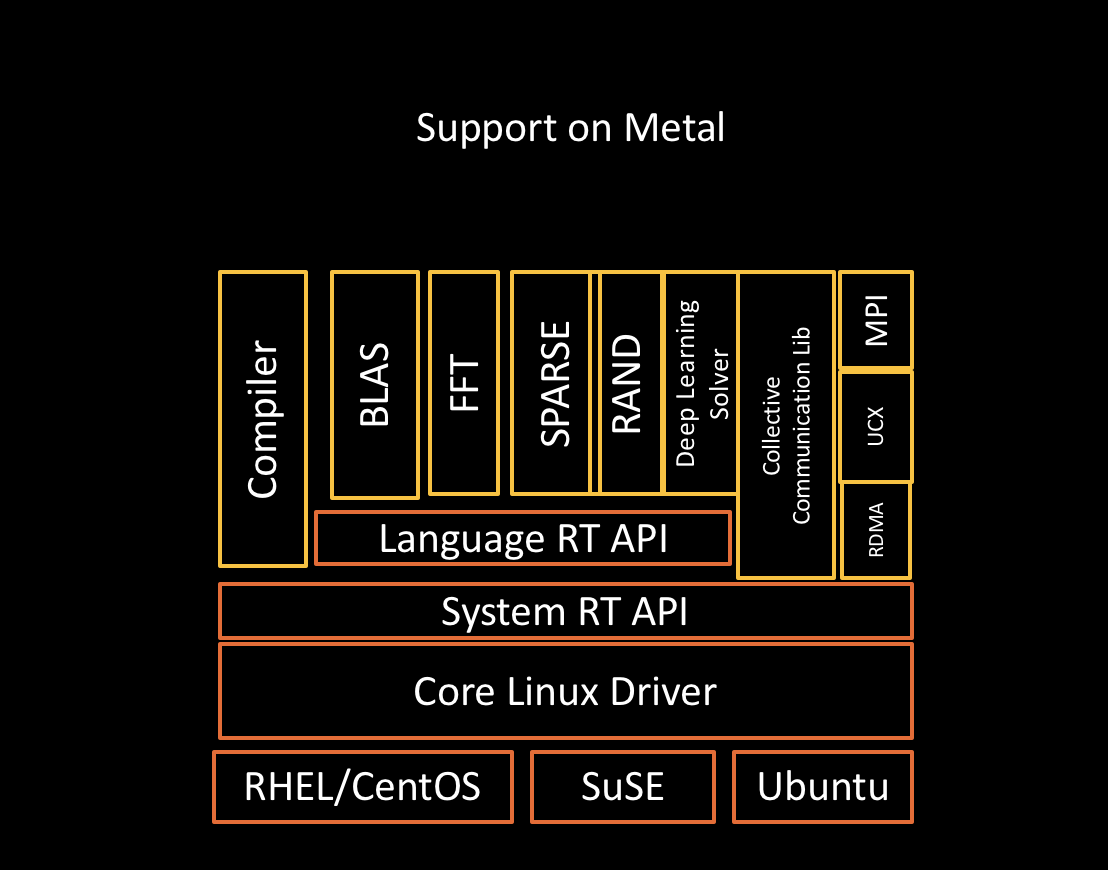
\includegraphics[height=.4\textwidth]{Figures/library.png}
    \caption{Soporte de librerías de ROCm}
    \label{fig:3}
\end{figure}

Respecto a la teoría que se utilizará para sostener las simulaciones a realizar, se seleccionó el método de Lattice Boltzman debido a su aceptación dentro del área de dinámica de fluidos y por el reciente aumento en su implementación sobre frameworks o software en general. 
Junto al método de Lattice Boltzmann base se considerarán condiciones de borde abiertas con tal de poder representar una continuidad de los fluidos.
Esto aumenta la utilidad de las simulaciones generadas, al asemejarlas aun más al comportamiento de fluidos en la vida real.
%asemejar los fluidos simulados a aquellos comportamientos en la vida real y por tanto la utilidad de las simulaciones generadas.
También, se espera poder plantear condiciones iniciales de diferentes simulaciones que permitan representar posibles tsunamis dentro de la costa Chilena (Figuras~\ref{fig:25}-\ref{fig:27}), esperando que sean un beneficio sobre la toma de decisiones al momento de la ocurrencia de uno después de la de un terremoto, pues como es de conocimiento publico, Chile es uno de los países más sísmicos del mundo junto con Japón~\cite{quake}.
Finalmente, uno de los legados principales de esta memoria será una implementación del método de Lattice Boltzmann en la plataforma ROCm, ya que, al ser esta un software sin un uso masificado, no presenta existencias de implementaciones de simulaciones de mecánica de fluidos en general.
\newpage
\secnumbersection{Estado del Arte}
\hlabel{sec:2}

A pesar de que, como fue mencionado anteriormente, AMD ROCm es una plataforma de desarrollo relativamente nueva, esto no ha detenido a diferentes investigadores de comenzar a utilizarla como forma de ampliar el hardware en el que se experimentan diferentes descubrimientos o trabajos científicos.

\subsection{ACELERACIÓN DE FACTORIZACIÓN SVD GPGPU}

En el año 2017, diferentes académicos de la Universidad de Tennessee, la Universidad de Manchester y el Laboratorio Nacional de Oak Ridge junto a un ingeniero de AMD trabajaron en la creación de rutinas BLAS de nivel 1, 2 y 3 para ser aplicadas en la aceleración de problemas pequeños de álgebra linear \cite{svd}.

El resultado final de dichas rutinas entregó una variación de la librería MAGMA, llamada MAGMA \textit{batched routines}, la cual corresponde a software sobre operaciones de álgebra linear optimizado a su uso en GPUs haciendo uso de operaciones por lotes, las cuales promueven la reutilización de datos, la minimización de operaciones y la maximización de ancho de banda.
La razón de utilizar la factorización SVD como modelo de pruebas, fue su gran cantidad de usos en aplicaciones tanto matemáticas como informáticas. 
Además, el uso particular de la versión bi-diagonal de la factorización, se debe 
a que esta se conforma por tres fases: de reducción, de solución y de transformación de vuelta, dentro de las cuales la primera corresponde a un 70\% o 90\% del tiempo total de computo, solo en operaciones de tipo BLAS.

El trabajo realizado se ejecutó finalmente en una GPU NVIDIA K420c GPU, para después portarse con la versión de HIP de aquel entonces a una GPU AMD Fiji Nano. Las características de cada una se ven en la tabla 1.

\begin{table}[h]
\centering
\caption{Descripción técnica de GPUs utilizadas en la aceleración de rutinas BLAS por lote.}
\begin{tabular}{cccc}
\hline
GPU       & \begin{tabular}[c]{@{}c@{}}Ancho de banda\\ {[}GB/s{]}\end{tabular} & \begin{tabular}[c]{@{}c@{}}Rendimiento máximo sobre DP\\ {[}Gflop/s{]}\end{tabular} & \begin{tabular}[c]{@{}c@{}}Tamaño de memoria\\ {[}GB{]}\end{tabular} \\ \hline
K40c      & 288                                                                 & 1430                                                                                & 12                                                                   \\
Fiji Nano & 512                                                                 & 512                                                                                 & 4                                                                    \\ \hline
\end{tabular}
\end{table}

Como se observa, la GPU de AMD (Fiji Nano) es inferior a la de NVIDIA (K40c) tanto en su rendimiento sobre operaciones de doble precisión (DP) como en el tamaño de su memoria, superando únicamente en la velocidad de escritura o lectura a su contra parte.
A pesar de esto, los resultados de las ejecuciones en ambas tarjetas para operaciones GEMV por lotes de tamaño 1000 sobre matrices cuadradas de tamaño progresivo tuvo resultados mucho más altos para la GPU de AMD, llegando a fluctuar entre 80 y 100 [Gflop/s] máximos, en comparación a la estabilización en 40 Gflop/s de la GPU de NVIDIA.

\begin{figure}[h]
\centering
\begin{subfigure}{.5\textwidth}
  \centering
  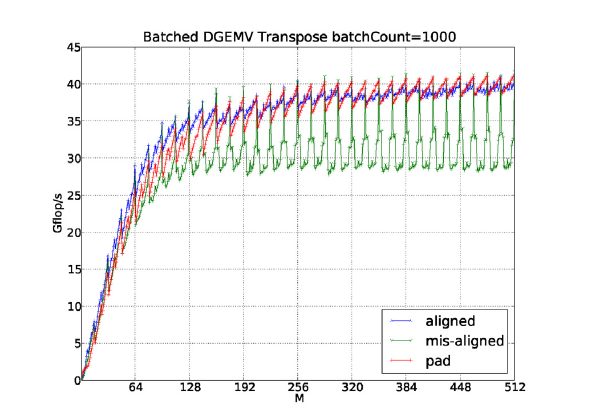
\includegraphics[width=.8\linewidth]{Figures/grap11.png}
  \caption{NVIDIA K40c}
\end{subfigure}%
\begin{subfigure}{.5\textwidth}
  \centering
  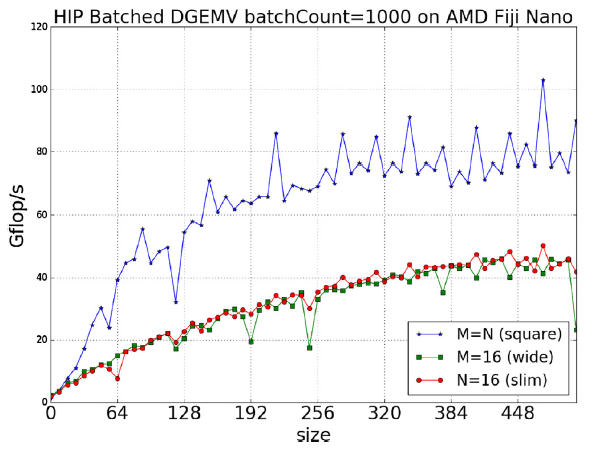
\includegraphics[width=.8\linewidth]{Figures/grap12.png}
  \caption{AMD Fiji Nano}
\end{subfigure}
\caption{Operaciones por segundo en la implementación de MAGMA con lotes de tamaño 1000 sobre matrices cuadradas de tamaño variable.}
\label{fig:4}
\end{figure}

\subsection{USO DE MOTORES DE INFERENCIA JUNTO AL FRAMEWORK \textit{FAST} PARA APLICACIONES MÉDICAS}

Durante el año 2019, un equipo de trabajo conformado por científicos investigadores del instituto médico tecnológico SINTEF en Noruega decidió desarrollar un software para su uso en diferentes aplicaciones médicas. 
Este estaba conformado por un variado conjunto de motores de inferencia, los cuales incluían 5 plataformas de trabajo sobre redes neuronales convolucionales: OpenVino 2019 R1, TensorRT y TensorFlow en tres versiones, sobre CPU, GPU NVIDIA (con cuDNN) y GPU AMD (con ROCm). Además, el equipo utilizó el framework FAST para visualización de imágenes y generación de una interfaz gráfica de aplicación \cite{fast}.

El software final, tiene 3 casos de prueba principales:
\begin{itemize}
    \item Segmentación en tiempo real de imágenes de ultra sonido; el cual corresponde a la localización de segmentos relevantes sobre un flujo grande de imágenes de ultra sonido, normalmente en blanco y negro y con ruido en su señal.
    \item Segmentación volumétrica de tomografías computarizadas; en el que se busca realizar una fragmentación sobre imágenes 3D resultantes de tomografías.
    \item Clasificación sobre parches de microscopía virtual; en donde se espera realizar clasificación de patrones en imágenes generadas por microscopio, cuya resolución ronda los 100k x 200k píxeles y su tamaño aproxima los 56 Gigabytes de datos.
\end{itemize}

En dichos casos, se realizaron diversas pruebas respecto al tiempo de ejecución de cada uno en todos los motores de inferencia que se utilizaron para la generación de la aplicación. 
Para el caso del uso de TensorFlow y TensorRT (desarrollado por NVIDIA para la generación de motores de inferencia sobre GPUs de la misma marca) se utilizó la tarjeta gráfica AMD Radeon R9 Fury para trabajar con ROCm y NVIDIA GTX 1080 ti para CUDA. 
En términos de las pruebas realizadas por caso, no se pudo realizar la segunda sobre segmentación volumétrica en tomografías sobre TensorFlow en ROCm por problemas de la versión de aquel entonces sobre el entrenamiento y evaluación de redes con convoluciones en 3D.
Las características principales de ambas GPUs y los resultados de los demás casos se pueden observar en las tablas 2 , 3 y 4 respectivamente.

\begin{table}[h]
\centering
\caption{Descripción técnica de GPUs utilizadas en implementación de software médico conformado por motor de interferencia más framework FAST.}
\begin{tabular}{cccc}
\hline
GPU         & \begin{tabular}[c]{@{}c@{}}Ancho de banda\\ {[}GB/s{]}\end{tabular} & \begin{tabular}[c]{@{}c@{}}Rendimiento máximo sobre DP\\ {[}Gflop/s{]}\end{tabular} & \begin{tabular}[c]{@{}c@{}}Tamaño de memoria\\ {[}GB{]}\end{tabular} \\ \hline
GTX 1080 ti & 288                                                                 & 1430                                                                                & 12                                                                   \\
R9 Fury     & 512                                                                 & 512                                                                                 & 4                                                                    \\ \hline
\end{tabular}
\end{table}

\begin{table}[h]
\centering
\caption{Tiempo de ejecución sobre segmentación de imágenes de ultra sonido, desde la carga de datos desde el disco hasta el procesamiento de 177 imágenes en la red neuronal. No incluye renderizado y está basado en 10 ejecuciones por motor de inferencia.}
\begin{tabular}{ccc}
\hline
Motor de inferencia & Procesador            & Tiempo de ejecución total {[}ms{]} \\ \hline
TensorFlow CPU      & Intel i5-4460         & 24193 \(\pm\) 1226                   \\
TensorFlow CUDA     & NVIDIA GTX 1080 ti    & 1547 \(\pm\) 17                      \\
TensorFlow ROCm     & AMD Radeon R9 Fury    & 2364 \(\pm\) 23                      \\
OpenVINO            & Intel HD Graphics 620 & 5898 \(\pm\) 26                      \\
TensorRT            & NVIDIA GTX 1080 ti    & 545 \(\pm\) 22                       \\ \hline
\end{tabular}
\end{table}

\begin{table}[h]
\centering
\caption{Tiempo de ejecución sobre clasificación de secciones en imágenes microscópicas, desde la carga de datos desde el disco hasta el procesamiento de la imagen completa. No incluye renderizado y está basado en 10 ejecuciones por motor de inferencia.}
\begin{tabular}{ccc}
\hline
Motor de inferencia & Procesador            & Tiempo de ejecución total {[}ms{]} \\ \hline
TensorFlow CPU      & Intel i5-4460         & 510564 \(\pm\) 1044                  \\
TensorFlow CUDA     & NVIDIA GTX 1080 ti    & 84684 \(\pm\) 1033                   \\
TensorFlow ROCm     & AMD Radeon R9 Fury    & 102594 \(\pm\) 269                   \\
OpenVINO            & Intel HD Graphics 620 & 581054 \(\pm\) 16304                 \\
TensorRT            & NVIDIA GTX 1080 ti    & 81298 \(\pm\) 180                    \\ \hline
\end{tabular}

\end{table}

A partir de estos resultados, se puede notar que la mayoría de los motores que utilizan como procesados una GPU tienen un tiempo de ejecución menor que aquellos que utilizan una CPU.
Si bien para este caso en particular, la GPU AMD fue sobrepasada por el uso del motor TensorRT, esto puede explicarse a que este corresponde a software desarrollado por NVIDIA específicamente para ser aplicado en inferencias y posee una optimización sobre el trabajo con aprendizaje profundo.

\subsection{PORTABILIDAD DE SOFTWARE SOBRE DINÁMICA MOLECULAR EN GPUS MODERNAS}

Dentro de la ciencia de materiales, se ha desarrollado un tipo de simulación para la representación de diferente conceptos mecánicos sobre diferentes tipos de partículas, la dinámica molecular.
Debido a la gran cantidad de fuerzas involucradas, es que la dinámica molecular es una de las simulaciones que más aplica el concepto de HPC.

El año 2020, un grupo de investigadores de diferentes casas de estudio en Rusia trabajaron respecto a como se comportaba el rendimiento de diferentes librerías de dinámica molecular sobre su transformación o porte desde CUDA a ROCm \cite{molecular}.
Particularmente, en el trabajo entregado solo se realizó dicha operación al programa LAMMPS (del inglés, Large-scale Atomic/Molecular Massively Parallel Simulator), software que permite la visualización del comportamiento de partículas dentro de un dominio limitado.
Si bien se trabajaron otros programas respecto a su rendimiento en las GPUs utilizadas, como HOOMD, GROMACS y OpenMM, estos no fueron portados usando las funcionalidades de ROCm, si no que o simplemente no poseían la capacidad de ser ejecutados por la GPU AMD o solo se transformaron a lenguaje OpenCL, el cual puede ser interpretado por GPUs de AMD, pero al tener un mayor nivel de abstracción no se trabaja de una manera óptima.
Para este experimento, se utilizó la GPU Titan V de NVIDIA y Radeon VII de AMD, cuyas especificaciones se pueden ver en la tabla siguiente.

\begin{table}[h]
\centering
\caption{Descripción técnica de GPUs utilizadas en ejecución de software de simulación computacional de dinámica molecular.}
\begin{tabular}{cccc}
\hline
GPU         & \begin{tabular}[c]{@{}c@{}}Ancho de banda\\ {[}GB/s{]}\end{tabular} & \begin{tabular}[c]{@{}c@{}}Rendimiento máximo sobre DP\\ {[}Gflop/s{]}\end{tabular} & \begin{tabular}[c]{@{}c@{}}Tamaño de memoria\\ {[}GB{]}\end{tabular} \\ \hline
%GTX 1080 ti & 484                                                                 & 354                                                                                & 11                                                                   \\
Titan V & 652                                                                 & 7450                                                                                & 12                                                                   \\
Radeon VII     & 1024                                                                 & 3360                                                                                 & 16                                                                    \\ \hline
\end{tabular}

\end{table}

En las pruebas realizadas, se simuló un liquido utilizando el modelo de potencial de Lennard-Jonnes, con un número de átomos variables desde $N = 55296$ a \(4000000\). Los resultados se pueden ver en el gráfico de la Figura~\ref{fig:5}. En esta, los cuadrados abiertos corresponden al resultado del uso del back-end en HIP de ROCm, mientras que los verdes corresponden al uso de CUDA.

A partir de los resultados encontrados, se concluyó de este trabajo que para la transformación realizada desde la versión de LAMMPS para CUDA hacia una versión ejecutable en AMD, se generaba un tiempo de ejecución por átomo por \textit{time step} del mismo orden de magnitud, dentro del rango entre $2.5 \times 10^{-8}$ y $1.3 \times 10^{-8}$ para un número de partículas $N > 10^6$.

\begin{figure}[ht]
    \centering
    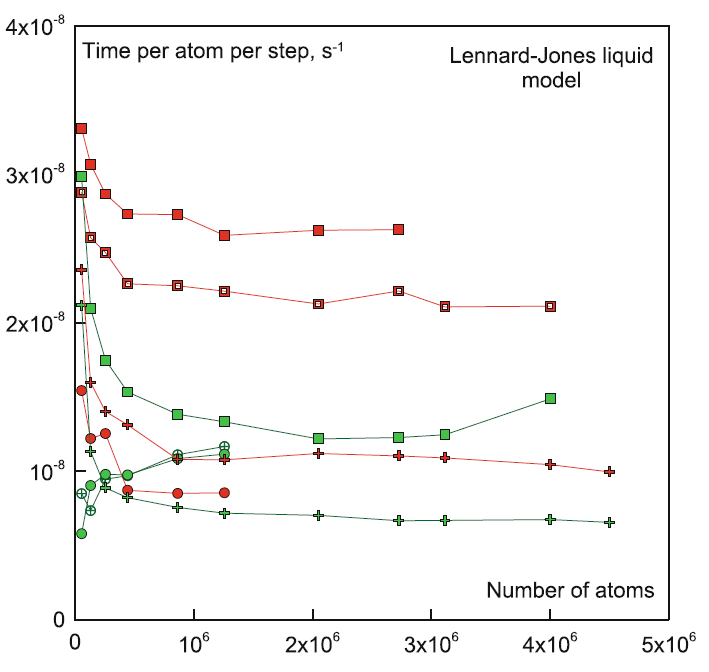
\includegraphics[height=.6\textwidth]{Figures/grap2.png}
    \caption{Tiempo de ejecución por átomo en la simulación computacional de dinámica molecular para un liquido al usar el modelo potencial de Lennard-Jonnes, en [$s^{-1}$].}
    \label{fig:5}
\end{figure}


\subsection{COMPARATIVA DEL SOPORTE EN TIEMPO REAL DE CARGAS EN PYTORCH}

Un equipo de trabajo conformado por académicos de la Universidad de Carolina del Norte en Estados Unidos de América, trabajó sobre la comparativa del rendimiento de diferentes \textit{benchmarks} de la biblioteca PyTorch, utilizado comúnmente para el entrenamiento de redes neuronales en aprendizaje profundo \cite{pytorch}.
Parte del articulo entregado, lista la siguiente serie de ventajas y desventajas del uso de la plataforma ROCm durante el tiempo de desarrollo:

\begin{itemize}
    \item Ventaja 1: El \textit{stack} de software proporcionado por AMD ROCm es \textit{open source} o de código abierto, lo cual implica que el código base esta abierto al publico general para su modificación~\cite{openS}.
    \item Ventaja 2: Programas actualmente presente en CUDA pueden ser transformados a una versión multiplataforma a través de HIP.
    \item Ventaja 3: El software base de bajo nivel en las GPUs AMD permite la partición de los núcleos de sus unidades de computo, lo cual permite una mayor atomicidad en la ejecución y generación de hebras, tanto para renderizado gráfico como para programación general.
    \item Desventaja 1: AMD ROCm solo soporta su uso en sistemas operativos Linux y en GPUs discretas, o las versiones modulares no integradas en placas madres.
    \item Desventaja 2: ROCm esta bajo constantes cambios de gran tamaño, lo cual se debe a su proceso actual de desarrollo.
    \item Desventaja 3: No hay una fuente de documentación oficial y centralizada de la plataforma, lo cual se conforma por cientos de miles de lineas de código.
\end{itemize}

A pesar de estos inconvenientes encontrados, el equipo no tuvo problemas en poder modificar el código de ROCm con tal de poder modificar la cantidad de unidades de computo asignado a las distintas colas de operaciones asignadas a y por la GPU.
Al parecer, este cambio de software de bajo nivel no es posible de implementar para la ejecución en NVIDIA, pues las GPUs de dicha marca no soportan el cambio de tamaño en las ``mascaras'' de unidades de computo a nivel de hardware.
Lo anterior serviría para poder limitar el poder de computo asignado a cada hilo generado.

Por último, para poder generar una comparativa del rendimiento generado por distintas GPUs, se corrió una red neuronal con pesos asignados por un entrenamiento previo con tal de clasificar imágenes de dígitos escritos a mano del conjunto de datos MNIST.
En esto, se utilizaron las GPUs NVIDIA Titan V, GTX 1060, GTX 970, AMD RX 570 y una CPU Intel Xeon 4110, cuyos tiempos de computo y especificaciones (de las tarjetas gráficas) se detallan en la tabla 6 y 7 respectivamente.

\begin{table}[h]
\centering
\caption{Tiempo de computo en la ejecución de una red neuronal para la clasificación de imágenes del conjunto de datos MNIST en [ms].}
\begin{tabular}{cccccc}
\hline
          & Mínimo & Máximo & Media & Promedio & Desviación Estándar \\ \hline
Titan V   & 0.51   & 5.79   & 0.51  & 0.52     & 0.08                \\
GTX 1060  & 1.40   & 1.63   & 1.42  & 1.42     & 0.01                \\
GTX 970   & 1.38   & 2.77   & 1.40  & 1.40     & 0.02                \\
RX 570    & 4.19   & 5.02   & 4.21  & 4.32     & 0.18                \\
Xeon 4110 & 5.54   & 18.43  & 8.60  & 8.40     & 1.78                \\ \hline
\end{tabular}

\end{table}

\begin{table}[h]
\centering
\caption{Descripción técnica de GPUs utilizadas en la ejecución de una red neuronal para la clasificación de imágenes del conjunto de datos MNIST.}
\begin{tabular}{cccc}
\hline
GPU         & \begin{tabular}[c]{@{}c@{}}Ancho de banda\\ {[}GB/s{]}\end{tabular} & \begin{tabular}[c]{@{}c@{}}Rendimiento máximo sobre DP\\ {[}Tflop/s{]}\end{tabular} & \begin{tabular}[c]{@{}c@{}}Tamaño de memoria\\ {[}GB{]}\end{tabular} \\ \hline
Titan V & 652                                                                 & 7.45                                                                                & 12                                                                   \\
GTX 1060 & 192                                                                 & 0.132                                                                                & 6                                                                   \\
GTX 970 & 224                                                                & 0.122                                                                                & 4                                                                   \\
RX 570     & 224                                                               & 0.318                                                                              & 4                                                                    \\ \hline
\end{tabular}

\end{table}

Cabe destacar que si bien los resultados anteriores reportan un menor rendimiento de la GPU AMD RX 570 en perspectiva con las GPUs de NVIDIA, esto se debe netamente al proceso activo de mejoras de la plataforma ROCm, pues en términos de características del hardware, esta está al mismo nivel que la NVIDIA GTX 1060.

En paralelo a los ejemplos de implementaciones realizadas para ambas marcas de tarjeta gráfica con tal de realizar una comparativa en rendimiento, no se pudo encontrar una investigación o caso de prueba que implemente específicamente el método de Lattice Boltzmann y que se ejecute al menos en una tarjeta AMD usando la plataforma ROCm.




\newpage
\secnumbersection{Desarrollo previo}
\hlabel{sec:3}

\subsection{COMPARATIVA TÉCNICA ENTRE TARJETAS GRÁFICAS.}

\hlabel{sec:3.1}

Para la experimentación realizada en las siguientes secciones de esta memoria, se utilizaron dos tarjetas gráficas, de NVIDIA y AMD respectivamente, que tienen especificaciones similares en termino de la gama a la que pertenecen respecto a su año de salida. 
Tomando lo anterior en cuenta, y debido al desabastecimiento general de tarjetas gráficas que ha sufrido el mercado tecnológico en los últimos años es que se escogió la GPU NVIDIA GTX 960M de arquitectura código Maxwell y AMD RX570 de arquitectura código Polaris.
Cabe destacar que la tarjeta GTX 960M estuvo enfocada en la venta de laptops de alto rendimiento~\cite{gtx960m} mientras que la tarjeta RX570 está pensada para computadoras personales de escritorio, ambas como partes de una gama media-alta en el mercado.

Como se mencionó anteriormente la GPU GeForce GTX 960M, lanzada al mercado el año 2015, corresponde a la a la primera generación de la arquitectura Maxwell, pues hace uso de un chip GM107.
Este chip esta compuesto por un Clúster de Proceso Gráfico (GPC, del ingles \textit{Graphic Processing Cluster}), dos controladores de memoria encargados del flujo de memoria entre CPU y GPU, 2 \textit{Megabyte} de memoria caché L2 y 16 Unidades de Salida de Renderizado (ROP), las cuales tienen como aplicación generar cálculos finales en el renderizado necesario para los programas que hagan uso de la GPU.
A su vez, el GPC está compuesto por 5 Multiprocesadores de Streaming (SM, del inglés \textit{Streaming Multiprocessor}) los cuales se conforman cada uno por un motor de Polimorfismo (del inglés \textit{Polymorph engine}) encargado de gestionar los recursos para el renderizado general, 8 motores de textura encargados del mapeo textura-modelo, \textit{Warp Schedulers} y núcleos CUDA (CU).
En esta arquitectura, la unidad básica de procesamiento corresponde al núcleo CUDA, y la unidad mínima de ejecución corresponde al \textit{Warp}.
En general, las tarjetas NVIDIA actuales consideran un \textit{Warp} como 32 hilos de ejecución, y en general la arquitectura Maxwell tiene la capacidad de enviar a cada núcleo 2 instrucciones por cada \textit{clock} de la tarjeta \cite{nwhitepaper}.
Una representación aproximada de los componentes listados se puede observar en la Figura~\ref{fig:6}.


\begin{figure}[h!]
    \centering
    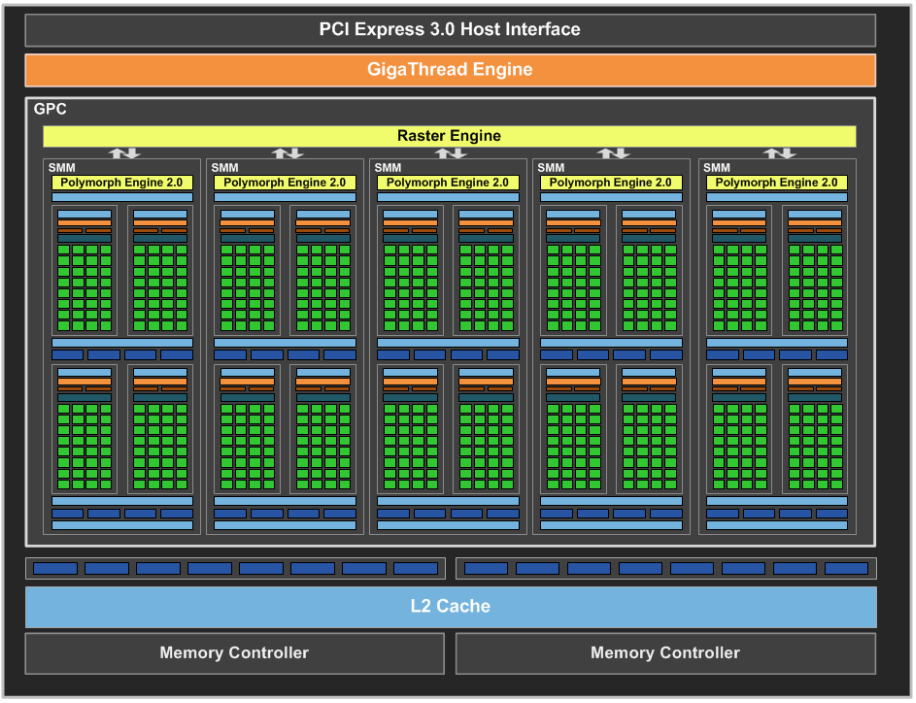
\includegraphics[width=.8\textwidth]{Figures/nvidia.png}
    \caption{Diagrama de bloque sobre arquitectura de chip GM107}
    \label{fig:6}
\end{figure}


Por otro lado, la GPU RX570 fue lanzada al mercado el año 2017 y corresponde a la arquitectura Polaris al usar un chip Polaris 20XL. 
La estructura general de esta arquitectura esta compuesta por un Procesador de Comandos Gráficos (del inglés, \textit{Graphics Command Processor}), distintos Motores de Computo Asíncrono (del inglés, \textit{Asynchronous Compute Engine }) y \textit{Hardware Scheduler} encargados de la gestión y ejecución asíncrona de ciertas llamadas a la GPU, y por último el conjunto de memoria L2 (de 2 \textit{Megabyte} para la tarjeta usada).
De la misma forma que el GPC en la tarjeta de NVIDIA, el Procesador de Comandos Gráficos se divide varios Motores de Sombreado (del inglés, \textit{Shader Engines}), que a su vez se dividen en distintas sub unidades, de las cuales destacan Procesadores Geométricos encargados del renderizado gráfico, y Unidades de Computo (del inglés, \textit{Compute Units}) las cuales corresponden a un conjunto de \textit{ROP's}, motores de textura y Procesadores de Sombreado (del inglés, \textit{Shader Processor}) \cite{awhitepaper}.
En la arquitectura Polaris, la unidad básica de procesamiento corresponde al \textit{Shader Processor}, y la unidad mínima de ejecución corresponde al \textit{Wavefront}.
Por definición, 16 \textit{Wavefronts} corresponden a un \textit{Workgroup} y cada \textit{Wavefront} esta conformado por 64 hilos de ejecución.
La Figura~\ref{fig:7} presenta una representación de la arquitectura y sus componentes listados.

\begin{figure}[h!]
    \centering
    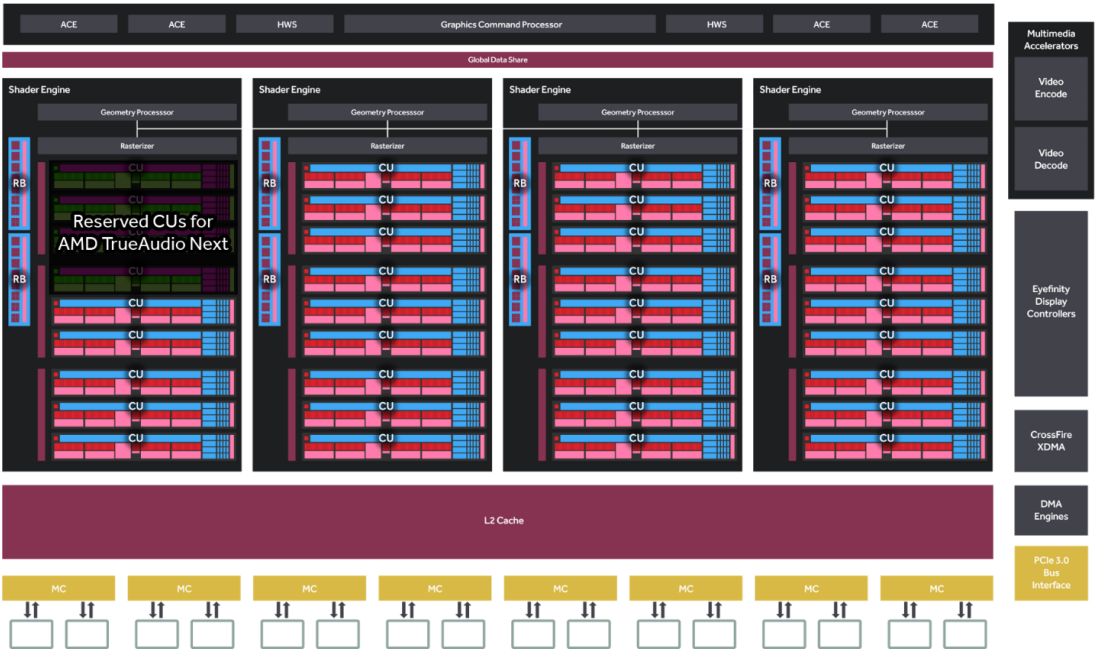
\includegraphics[width=.8\textwidth]{Figures/amd.png}
    \caption{Diagrama de bloque sobre arquitectura de chip Polaris 10}
    \label{fig:7}
\end{figure}

Además de las unidades estructurales presentes en ambas tarjetas, se deben tomar en cuenta que existen muchas otras características agregadas por cada compañía para solventar las necesidades de computo gráfico que existe en el nicho de venta, tales como unidades extra para el computo de teselado, texturas o iluminación con mejor rendimiento, una mayor ganancia a menor uso de voltaje, o soporte para diferentes APIs ligadas al rendimiento de aplicaciones, tales como DirectX o Vulkan~\cite{directx, vulkan}.
Presentando otro ejemplo, el \textit{whitepaper} de la arquitectura Polaris publicado por AMD menciona la capacidad de los controladores de las tarjetas gráficas de poder reservar unidades de procesamiento para tareas especificas, tales como procesado de audio.
Estas pueden ser oportunidades que permitan extender el dominio de la programación paralela en GPU, sin embargo, tomando en cuenta que solamente interesan aquellas propiedades que influyan directamente con la ejecución de códigos de programación paralela en GPU se omitirán por simplicidad. 
A continuación se presenta una tabla comparativa de las especificaciones de ambas tarjetas gráficas en torno a características generales, configuraciones de renderizado y rendimiento teórico sobre operaciones de punto flotante.

% Tabla V3
\renewcommand{\arraystretch}{1.5}
\begin{table}[ht!]
\centering
\caption{Comparación de especificaciones técnicas de tarjetas AMD RX570 y NVIDIA GTX960M.}
\begin{tabularx}{\textwidth}{XX|c|c|}
\cline{3-4}
                                                                    &                         & AMD RX570             & NVIDIA GTX960M        \\ \hline
\multicolumn{1}{|l|}{\multirow{2}{*}{Rendimiento Teórico}}          & FP32 (float)            & \(5.095\) {[}Tflop/s{]} & \(1.505\) {[}Tflop/s{]} \\ \cline{2-4} 
\multicolumn{1}{|l|}{}                                              & FP64 (double)           & \(318.5\) {[}Gflop/s{]} & \(47.04\) {[}Gflop/s{]} \\ \hline
\multicolumn{1}{|l|}{\multirow{3}{*}{Configuración de Renderizado}} & Unidades de Sombreado   & 2048 {[}SP{]}         & 640 {[}CU{]}          \\ \cline{2-4} 
\multicolumn{1}{|l|}{}                                              & Unidades de Texturizado & 128 {[}TMU{]}         & 40 {[}TMU{]}          \\ \cline{2-4} 
\multicolumn{1}{|l|}{}                                              & ROPs                    & 16 {[}ROP{]}          & 32c {[}ROP{]}         \\ \hline
\multicolumn{1}{|l|}{\multirow{3}{*}{Especificaciones Generales}}   & Clock Base              & 1168 {[}MHz{]}        & 1097 {[}MHz{]}        \\ \cline{2-4} 
\multicolumn{1}{|l|}{}                                              & Tamaño de Memoria       & 4 {[}GB{]}            & 8 {[}GB{]}            \\ \cline{2-4} 
\multicolumn{1}{|l|}{}                                              & Anchos de Banda         & \(224.0\)  {[}GB/s{]}   & \(80.19\) {[}GB/s{]}    \\ \hline
\end{tabularx}
\end{table}

\iffalse

%Tabla V2

\begin{table}[ht!]
\centering
\caption{Comparación de especificaciones técnicas de tarjetas AMD RX570 y NVIDIA GTX960M.}
\begin{tabular}{ll|c|c|}
\cline{3-4}
                                                                                             &                         & AMD RX570    & NVIDIA GTX960M \\ \hline
\multicolumn{1}{|l}{\begin{tabular}[c]{@{}l@{}}Rendimiento \\ Teorico\end{tabular}}          & FP32 (float)            & 5.095 TFLOPS & 1.505 TFLOPS   \\
\multicolumn{1}{|l}{}                                                                        & FP64 (double)           & 318.5 GFLOPS & 47.04 GFLOPS   \\ \hline
\multicolumn{1}{|l}{\begin{tabular}[c]{@{}l@{}}Configuración\\  de Renderizado\end{tabular}} & Unidades de Sombreado   & 2048 SP      & 640 CU         \\
\multicolumn{1}{|l}{}                                                                        & Unidades de Texturizado & 128 TMU      & 40 TMU         \\
\multicolumn{1}{|l}{}                                                                        & ROPs                    & 16 ROPs      & 32 ROPs        \\ \hline
\multicolumn{1}{|l}{General}                                                                 & Clock Base              & 1168 MHz     & 1097 MHz       \\
\multicolumn{1}{|l}{}                                                                        & Tamaño de Memoria       & 4 GB         & 4 GB           \\
\multicolumn{1}{|l}{}                                                                        & Ancho de Banda          & 224.0 GB/s   & 80.19 GB/s     \\ \hline
\end{tabular}
\end{table}



% Tabla V1

\begin{table}[h!]
\centering
\begin{tabular}{ll|c|c|}
\cline{3-4}
                                                  &                         & AMD RX570    & NVIDIA GTX960M \\ \hline
\multicolumn{1}{|l}{Rendimiento \newline Teórico}          & FP32 (float)            & 5.095 TFLOPS & 1.505 TFLOPS   \\
\multicolumn{1}{|l}{}                             & FP64 (double)           & 318.5 GFLOPS & 47.04 GFLOPS   \\ \hline 
\multicolumn{1}{|l}{Configuración de Renderizado} & Unidades de Sombreado   & 2048 SP      & 640 CU         \\
\multicolumn{1}{|l}{}                             & Unidades de Texturizado & 128 TMU      & 40 TMU         \\
\multicolumn{1}{|l}{}                             & ROPs                    & 16 ROPs      & 32 ROPs        \\ \hline
\multicolumn{1}{|l}{Características Generales}                      & Clock Base              & 1168 MHz     & 1097 MHz       \\
\multicolumn{1}{|l}{}                             & Tamaño de Memoria       & 4 GB         & 4 GB           \\
\multicolumn{1}{|l}{}                             & Ancho de Banda          & 224.0 GB/s   & 80.19 GB/s     \\ \hline
\end{tabular}
\caption{Comparación de especificaciones técnicas de tarjetas AMD RX570 y NVIDIA GTX960M}
\end{table}

\fi

\subsection{PROGRAMACIÓN EN ROCM Y COMPARATIVA A CUDA}

\hlabel{sec:3.2}

Antes de realizar cualquier tipo de acercamiento a la solución del problema propuesto, se deben mencionar algunos términos claves en el paradigma de programación paralela presente en las plataformas de desarrollo que se compararán, específicamente Instrucción Única y Múltiples Hilos (del inglés, \textit{Single Instruction Multiple Thread} o \textit{SIMT}).
El modelo \textit{SIMT} corresponde a una combinación del \textit{Multithreading} y \textit{Single Instruction Multiple Data}, una clasificación dentro de la Taxonomía de Flynn \cite{simt} de arquitectura de computadoras, la cual implica que una sola instrucción puede entregarse a distintas unidades de procesamiento para su ejecución simultanea.
Una serie de instrucciones ejecutadas es lo que se conoce como ``hilo'' o \textit{thread} y múltiples \textit{threads} que trabajan de forma paralela es lo que se llama como \textit{multithreading}.
Tomando en cuenta el modelo \textit{SIMT}, es que se trabaja con ambas plataformas de desarrollo (ROCm y CUDA), en las cuales cada una posee APIs representadas por métodos que facilitan la gestión de dispositivos (o tarjetas gráficas), eventos, tipos de memoria a utilizar (global o compartida), o librerías para trabajos específicos del área de HPC, presentados brevemente en el Capítulo~\hyperref[sec:1]{1}.

Dentro del dominio de la programación en CUDA y ROCm existe el termino ``kernel'', el cual corresponde a una encapsulación de instrucciones con forma de función la cual será enviada a la GPU con tal de ser ejecutada.
Parte de lo que se tiene que tomar en cuenta al momento de realizar programación paralela y por consecuencia en la definición de un kernel, son principalmente:

\begin{itemize}
    \item Condiciones de carrera, lo cual toma en cuenta que antes de comenzar con un nuevo conjunto de instrucciones (o kernel) todos los \textit{threads} comenzados con anterioridad deben terminar.
    \item Exclusión mutua, cuya idea es mantener la coherencia de datos al momento de usar recursos compartidos, o leer/escribir en memoria global.
\end{itemize}

\subsubsection{Suma de vectores}

Para poner un ejemplo, se podría pensar en la tarea de realizar una operación entre vectores, ya sea suma, producto interno o cualquier otro tipo de función \textit{element wise} o elemento a elemento.
En este caso no es necesario considerar las condiciones de carrera, pues la instrucción es una sola, sin embargo, lo que si hay que planear es el dominio de trabajo de cada \textit{thread}, por lo que si se utilizaran \(n\) \textit{threads} para realizar la suma de dos vectores de tamaño \(m\), cada \textit{thread} $i \in [ 0, n-1]$ tendría que trabajar netamente con los valores desde la posición $\left \lfloor{\frac{m}{n}}\right \rfloor  i$ hasta la posición $\left \lfloor{\frac{m}{n}}\right \rfloor i+1$.
Esto se puede esquematizar en el pseudo código del Algoritmo~\ref{alg:1}.
\begin{algorithm}
\caption{Kernel - Suma de vectores}
\label{alg:1}
\begin{algorithmic}[1]
\Procedure{VectorAdd}{vector1, vector2, vector3, m, n}
\State $i \leftarrow$ número de \textit{thread}
\State $j = \frac{m}{n} i$  
\For {j <  $\frac{m}{n} i + 1$}
    \State vector3[j] = vector1[j] + vectror2[j]
\EndFor
\EndProcedure
\end{algorithmic}
\end{algorithm}

Hasta hace algunos año una de las plataforma de HPC más utilizada era CUDA y es por esto que en posterior al lanzamiento de ROCm estuviera justificado la forma que tendría su forma de aplicación. 
Actualmente ROCm funciona en base al lenguaje C++ junto al dialecto \textit{Heterogeneous-Computing Interface for Portability} (HIP) el cual comprende una amplia gama de APIs para el aprovechamiento de los núcleos de procesamiento de tarjetas AMD, que a su vez poseen similitud en nombre y soporte para un sub conjunto de las funciones de CUDA.
Por estos motivos es que junto a HIP, ROCm presenta la herramienta Hipify, la cual corresponde a un programa que permite analizar gramaticalmente archivos de código de CUDA para generar código en C++ compilable por HIP.
Cabe destacar que existen dos variantes de este software, una en base al lenguaje Perl y otra en base al front end para compilaciones Clang, de los cuales se pueden obtener ventajas y desventajas de cada una. 
La principal ventaja de Hipify-Clang, es que al ser un traductor, realiza una revisión sintáctica de el o los archivos de entrada, lo cual indica en momento de ejecución si la traducción fue correcta o no. 
Esta misma característica de la versión en Clang es su mayor desventaja, pues si el código en CUDA C está incorrecto o fuera de los limites del software no se generará un programa en HIP.
Por otro lado, Hipify-Perl corresponde a una implementación en base a expresiones regulares, más directa en comparación a su contra parte, la cual siempre generará código de HIP independiente de su correctitud.
Además, una última desventaja de la versión de Perl es la falta de soporte a ciertas funciones de CUDA C \cite{HIP}.


Haciendo uso del ejemplo previo se presenta la Figura~\ref{fig:8}, la cual contiene la definición del kernel \textit{vectorAdd} como implementación del Algoritmo~\ref{alg:1}.
En este caso, se está considerando que al momento de ejecutar el kernel se hará con una configuración que genere un \textit{thread} por cada elemento del vector final en el que se almacenará la suma y debido a esto es que existe diferencia entre la linea 3-4 del Algoritmo~\ref{alg:1} y la condicional en la linea 7 del código de la Figura~\ref{fig:8}, además de los parámetros de entrada en cada uno.

\begin{figure}[h!]
\centering
\begin{lstlisting}[language=C, frame=single, breaklines=true, numbers=left, style=CudaStyle ]
__global__ void
vectorAdd(const float *A, const float *B, 
            float *C, int numElements)
{
    int i = blockDim.x * blockIdx.x + threadIdx.x;
    if (i < numElements)
    {
        C[i] = A[i] + B[i];
    }
}
\end{lstlisting}
\caption{Definición de kernel para suma de vectores.}
\label{fig:8}
\end{figure}

El código presentado en la Figura~\ref{fig:9} corresponde a una versión simplificada de la función principal {\verb main() } del archivo vectorAdd.cu presente en los ejemplos de la versión 11.2 del \textit{CUDA Toolkit} \cite{samples}.
La estructura en este corresponde a la siguiente:
\begin{itemize}
    \item \textbf{Lineas 5-10}: Configuración de tamaño de los 3 arreglos (representación de vectores) necesarios y su asignación de memoria respectiva.
    \item \textbf{Lineas 11-15}: Inicialización de ambos arreglos a sumar con números tipo \textit{float} aleatorios.
    \item \textbf{Lineas 16-23}: Definición de los 3 punteros a los arreglos necesarios en memoria de GPU, su asignación de memoria respectiva y la copia de datos desde memoria de CPU a GPU.
    \item \textbf{Lineas 25-27}: Calculo del número de \textit{threads} a utilizar en GPU y ejecución del kernel presentado en el Algoritmo~\ref{alg:1}. Para esta instancia en particular (pues el tamaño del arreglo esta asignado arbitrariamente a 5000), el número total de \textit{threads} será igual a $256\times \text{blocksPerGrid} = 256 \times (5000 + 256 - 1) \div 256 = 5255$ [\textit{thread}].
    \item \textbf{Lineas 29-36}: Copia de resultados del kernel al arreglo respectivo en CPU y liberación de memoria en CPU y GPU para evitar perdidas de memoria o \textit{memory leaks}.
\end{itemize}

En contraste con lo anterior, la Figura~\ref{fig:10} presenta la salida de ejecutar la herramienta \textit{Hipify} en su versión basada en Perl con el código de la Figura~\ref{fig:9} como entrada.
Haciendo énfasis en los cambios realizados por \textit{Hipify}, se deben destacar las lineas, (17, 18, 19), (22, 23, 27), 27 y (31, 32, 33) en las cuales se realizan asignaciones de memoria, se hacen transferencias de datos entre memoria de CPU y GPU, se ejecuta el kernel y se libera memoria, todo en GPU y tan solo cambiando la firma de los métodos utilizados por CUDA con su contra parte en HIP. 
El resultado de la ejecución de ambos kernel en tarjetas gráficas de AMD y NVIDIA para diversos tamaños de vectores se presentará en el Capítulo~\hyperref[sec:4]{4}.


\newpage

\begin{figure}[h!]
\centering
\begin{lstlisting}[language=C++, frame=single, breaklines=true,style=CudaStyle, basicstyle=\footnotesize, numbers=left]
#include <stdio.h>
#include <cuda_runtime.h>
int main(int argc, char* argv[])
{
    int numElements = 50000;
    size_t size = numElements * sizeof(float);
    
    float *h_A = (float *)malloc(size);
    float *h_B = (float *)malloc(size);
    float *h_C = (float *)malloc(size);
    for (int i = 0; i < numElements; ++i)
    {
        h_A[i] = rand()/(float)RAND_MAX;
        h_B[i] = rand()/(float)RAND_MAX;
    }
    float *d_A = NULL;
    cudaMalloc((void **)&d_A, size);
    float *d_B = NULL;
    cudaMalloc((void **)&d_B, size);
    float *d_C = NULL;
    cudaMalloc((void **)&d_C, size);
    cudaMemcpy(d_A, h_A, size, cudaMemcpyHostToDevice);
    cudaMemcpy(d_B, h_B, size, cudaMemcpyHostToDevice);

    int threadsPerBlock = 256;
    int blocksPerGrid =(numElements + threadsPerBlock - 1) / threadsPerBlock;
    vectorAdd<<<blocksPerGrid, threadsPerBlock>>>(d_A, d_B, d_C, numElements);

    cudaMemcpy(h_C, d_C, size, cudaMemcpyDeviceToHost);

    cudaFree(d_A);
    cudaFree(d_B);
    cudaFree(d_C);
    free(h_A);
    free(h_B);
    free(h_C);

    printf("Done\n");
    return 0;
}
\end{lstlisting}
\caption{Función main()  de un código CUDA para suma de vectores vectorAdd.cu.}
\label{fig:9}
\end{figure}

\newpage

\begin{figure}[h!]
\centering
\begin{lstlisting}[language=C++, frame=single, breaklines=true,basicstyle=\footnotesize, numbers=left, style=CudaStyle]
#include <stdio.h>
#include <hip/hip_runtime.h>
int main(int argc, char* argv[])
{
    int numElements = 50000;
    size_t size = numElements * sizeof(float);
   
    float *h_A = (float *)malloc(size);
    float *h_B = (float *)malloc(size);
    float *h_C = (float *)malloc(size);
    for (int i = 0; i < numElements; ++i)
    {
        h_A[i] = rand()/(float)RAND_MAX;
        h_B[i] = rand()/(float)RAND_MAX;
    }
    float *d_A = NULL;
    hipMalloc((void **)&d_A, size);
    float *d_B = NULL;
    hipMalloc((void **)&d_B, size);
    float *d_C = NULL;
    hipMalloc((void **)&d_C, size);
    hipMemcpy(d_A, h_A, size, hipMemcpyHostToDevice);
    hipMemcpy(d_B, h_B, size, hipMemcpyHostToDevice);

    int threadsPerBlock = 256;
    int blocksPerGrid =(numElements + threadsPerBlock - 1) / threadsPerBlock;
    hipLaunchKernelGGL(vectorAdd, dim3(blocksPerGrid), dim3(threadsPerBlock), 0, 0, d_A, d_B, d_C, numElements);
    hipMemcpy(h_C, d_C, size, hipMemcpyDeviceToHost);

    
    hipFree(d_A);
    hipFree(d_B);
    hipFree(d_C);
    free(h_A);
    free(h_B);
    free(h_C);

    printf("Done\n");
    return 0;
}
\end{lstlisting}
\caption{Función  main()  de un código compilable por HIP, resultado de la ejecución de la herramienta Hipify-Perl en el código de la Figura~\ref{fig:9}.}
\label{fig:10}
\end{figure}
\newpage

\subsubsection{Multiplicación de matrices}

Un marco referencial muy utilizado con tal de poder entender y así poner a prueba la programación paralela usando GPU es la multiplicación de matrices.
Considerando dos matrices $A, B \in \mathbb{R}^{n\times n}$, su multiplicación daría como resultado una matriz $C\in R^{n\times n}$ en la que el valor de cada coeficiente estaría dado por la formula,
\begin{equation*}
    c_{ij} = a_{i1}b_{1i} + a_{i2}b_{2i} + \dots + a_{in}b_{ni} = \sum_{k=1}^n a_{ik}b_{ki}
\end{equation*}
en donde $i, j \in [0,n]$ y \(a_{ij}\), \(b_{ij}\), \(c_{ij}\) corresponden a coeficientes de $A, B, C$ respectivamente.

En un principio, esto podría realizarse de forma secuencial y de manera exhaustiva realizando productos internos (ver Figura~\ref{fig:11}) entre la combinatoria de todas las filas y columnas de las matrices \(A\) y \(B\).

\begin{figure}[h!]
\centering
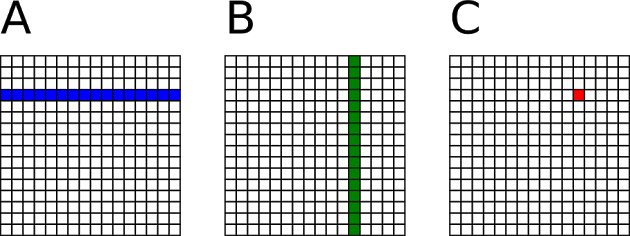
\includegraphics[width=0.8\textwidth]{Figures/naive.png}
\caption{Esquema de procedimiento común en una multiplicación de matrices con implementación secuencial, fuente:~\cite{matrixM}.}
\label{fig:11}
\end{figure}

Ahora, haciendo uso de una implementación en programación paralela y la ejecución en una GPU, se podría replicar lo propuesto a la hora de realizar la suma de dos vectores en la sección anterior, asignando a cada \textit{thread} la tarea de realizar uno de los productos internos, por lo que el total de \textit{threads} tendría que ser igual o mayor al número de elementos de la matriz resultante \(C\).
Esto se puede esquematizar en la definición de la función {\verb main() } y kernel propuestos en los Algoritmo~\ref{alg:2},\ref{alg:3}.

\begin{algorithm}
\caption{Función main()  - Multiplicación de matrices}
\label{alg:2}
\begin{algorithmic}[1]
%\algsetup{linenosize=<size>}
\Procedure{main}{}
\State definir A, B, C en la memoria de CPU
\State inicializar A, B
\State definir Agpu, Bgpu, Cgpu en la memoria de GPU
\State copiar memoria de A a Agpu
\State copiar memoria de B a Bgpu
\State definir cantidad de \textit{threads} en \(i\)
\State matrixMul<<i>>(Agpu, Bgpu, Cgpu)
\State copiar memoria de Cgpu a C
\EndProcedure
\end{algorithmic}
\end{algorithm}

\begin{algorithm}
\caption{Kernel - Multiplicación de matrices}
\label{alg:3}
\begin{algorithmic}[1]
%\algsetup{linenosize=<size>}
\Procedure{matrixMul}{Agpu, Bgpu, Cgpu}
\State definir tmp
\State calcular fila y columna de Cgpu en la que se trabajará (i,j)
\For {k = [0,n-1]}
    \State tmp = tmp + Agpu(k, j)*Bgpu(i, k)
\EndFor
\State Cgpu(i,j) = tmp
\EndProcedure
\end{algorithmic}
\end{algorithm}

Antes de continuar con las siguientes optimizaciones posibles para un algoritmo de multiplicación de matrices, se debe hacer la distinción entre lo que implica el uso de memoria global y memoria compartida.
La memoria global corresponde a registro accesibles por todas las unidades de procesamiento presentes en una GPU, mientras que la memoria compartida hace referencia a aquella que se puede acceder y es ``visible'' por \textit{threads} de un mismo bloque.
En este contexto, bloque hace referencia a la jerarquía de generación de threads de CUDA C y HIP, partiendo por una grilla, compuesta por bloques y que a su vez esta compuesta por cierta cantidad de \textit{threads}.
Estas abstracciones son partes de los parámetros presentes al momento de ejecutar un kernel, los cuales definen la cantidad total de \textit{threads}.

Para evitar limitaciones en el rendimiento de este algoritmo (más conocido como cuello de botella o \textit{bottle neck}) es que se le puede realizar una optimización utilizando \textit{Tiling}, o la división de la matriz final en bloques de tamaño arbitrario con tal de transferir la información de las matrices a las que se debe acceder a memoria compartida por \textit{threads} de un mismo grupo de trabajo, la cual se caracteriza por ser de acceso mucho más rápido.

Si bien con esto se pierde un poco de tiempo haciendo la transferencia de datos, la recompensa es mucho mayor por el acceso directo a los elementos de las matrices \(A\) y \(B\) a la hora de calcular los productos punto.
En este nuevo esquema y en las siguientes optimizaciones que se presentarán, el único cambio se encuentra en el código del kernel, por lo cual solo se realizarán actualizaciones del mismo.
En el pseudo código del Algoritmo~\ref{alg:4} sintetiza lo planteado, en donde, si se toma como ejemplo el diagrama de la Figura~\ref{fig:12}, se entiende que para ese caso la cantidad de \textit{Tiles} es igual a 2.
Así, en el primer ciclo for de la linea 6 del Algoritmo~\ref{alg:4}, cada thread encargado de generar \(C_{0,0}\) trabajará en trasladar a memoria compartida los elementos de la sub matriz \(A_{0,0}\) y \(B_{0,0}\) para generar una respuesta parcial y sincronizar, cosa que corresponde a generar una barrera que espera a que todos los \textit{threads} terminen sus instrucciones.
Luego, en la segunda iteración (y final para este caso), el grupo de \textit{threads} encargados de calcular \(C_{0,0}\) cargarán en memoria compartida \(A_{0,1}\) y \(B_{1,0}\), para obtener el resultado completo.


\begin{algorithm}
\caption{Kernel - Multiplicación de matrices}
\label{alg:4}
\begin{algorithmic}[1]
%\algsetup{linenosize=<size>}
\Procedure{matrixMul}{Agpu, Bgpu, Cgpu}
\State definir tamañoTile
\State definir A\_tile, B\_tile en memoria compartida
\State calcular fila y columna de Cgpu en la que se trabajará (i,j)
\State definir tmp
\For {tileIdx = [0, $n \div $tamañoTile]}
    \State calcular fila y columna de A\_Tile/B\_Tile en la que se trabajará (a,b)
    \State asignar valor correspondiente desde Agpu a A\_Tile 
    \State asignar valor correspondiente desde Bgpu a B\_Tile 
    \State sincronizar \textit{threads}
    \For {k = [0, tamañoTile]}
        \State tmp = tmp + A\_Tile(k, b) + B\_Tile(a, k)
    \EndFor
    \State sincronizar \textit{threads}
\EndFor
\State Cgpu(i,j) = tmp
\EndProcedure
\end{algorithmic}
\end{algorithm}

\begin{figure}[h!]
\centering
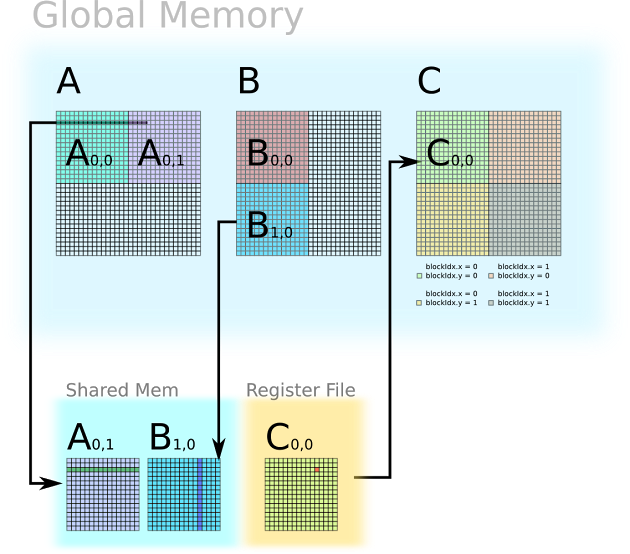
\includegraphics[width=0.8\textwidth]{Figures/opt1.png}
\caption{Esquema de implementación paralela para multiplicación de matrices usando \textit{Tiling}, fuente:~\cite{matrixM}.}
\label{fig:12}
\end{figure}

La coalescencia de memoria o \textit{memory coalescing} corresponde a un termino de la programación paralela en GPU la cual se refiere a un acceso ordenado a los segmentos de memoria que posee la tarjeta con la que se trabaja.
Esto ocurre, pues cada vez que se realiza un acceso a memoria por parte de un \textit{warp} o wavefront (conjunto de \textit{threads}), este debe ser respecto a un bloque de memoria contiguo.
Por tanto, si en una instrucción se debe acceder a celdas de memorias que se encuentran en sectores lejanos, el número de accesos es mayor y en consecuencia, más costoso computacionalmente.

Así, una solución para este problema es trasponer la matriz B al momento de trasladar los datos desde memoria global a memoria compartida, lo cual se puede implementar como un cambio en la linea 9 y 12 del Algoritmo~\ref{alg:5} respecto del Algoritmo~\ref{alg:4}. 

\begin{algorithm}
\caption{Kernel - Multiplicación de matrices con \textit{memory coalescing}}
\label{alg:5}
\begin{algorithmic}[1]
%\algsetup{linenosize=<size>}
\Procedure{matrixMul}{Agpu, Bgpu, Cgpu}
\State definir tamañoTile
\State definir A\_tile, B\_tile en memoria compartida
\State calcular fila y columna de Cgpu en la que se trabajará (i,j)
\State definir tmp
\For {tileIdx = [0, $n \div $tamañoTile]}
    \State calcular fila y columna de A\_Tile/B\_Tile en la que se trabajará (a,b)
    \State asignar valor correspondiente desde Agpu a A\_Tile 
    \State asignar valor correspondiente desde Bgpu a B\_Tile // de forma traspuesta 
    \State sincronizar \textit{threads}
    \For {k = [0, tamañoTile]}
        \State tmp = tmp + A\_Tile(k, b) + B\_Tile(k, a)
    \EndFor
    \State sincronizar \textit{threads}
\EndFor
\State Cgpu(i,j) = tmp
\EndProcedure
\end{algorithmic}
\end{algorithm}

Finalmente, sumado a las variantes de código explicadas, se puede analizar la cantidad de operaciones de bajo nivel que se designan al momento de compilar el archivo binario. 
En la arquitectura de unidades de procesamiento (al menos la presente en Maxwell) solo se permite realizar un operando entre elementos almacenados en la memoria compartida, lo cual se contra resta con el producto interno, el cual necesita una suma y una multiplicación en cada iteración del arreglo en memoria compartida (linea 12 del Algoritmo~\ref{alg:5}).
Esto podría ser solucionado utilizando memoria global para alguna de las dos matrices, pero con esta medida se perdería parte del trabajo realizado por el \textit{Tiling} en la primera variante.
Entonces, una alternativa viable es utilizar el producto externo en vez del producto interno.
Este se define a partir de la formula,

\begin{equation*}
u \otimes v = 
\begin{bmatrix} 
	u_1v_1 & u_1v_2 & \dots & u_1v_n\\
	u_2v_1 & u_2v_2 & \dots & u_2v_n\\
	\vdots & \vdots & \ddots & \vdots \\
	u_mv_1 & u_mv_2 & \dots & u_mv_n\\
	\end{bmatrix}
\end{equation*}



en donde $u\in R^m$ y $v\in R^n$.
De acuerdo a esta definición, por consecuencia la multiplicación de dos matrices \(A\) y \(B\) esta definida por,
\begin{equation*}
    C = A\,B = \sum_{i=1}^n a_i \otimes b^T_i
\end{equation*}
en la cual \(a_i\) es la i-esima columna de \(A\) y $b_i^T$ es la i-esima fila de \(B\).

Para poder aplicar el producto externo junto al \textit{Tiling}, se debe implementar el traspaso de datos de tan solo la matriz \(A\) a la memoria compartida del tamaño de un \textit{Tile} y realizar la operatoria con toda una fila de \(B\), como se ejemplifica en la Figura~\ref{fig:13}.

\begin{figure}[h!]
\centering
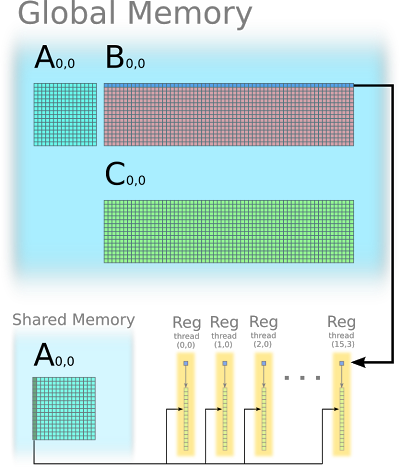
\includegraphics[width=0.8\textwidth]{Figures/opt2.png}
\caption{Esquema de implementación paralela para multiplicación de matrices usando \textit{Tiling} y el producto externo, fuente:~\cite{matrixM}.}
\label{fig:13}
\end{figure}

En el Algoritmo~\ref{alg:6}, se incluye el pseudo código de lo que sería una implementación de multiplicación de matrices aplicando todas las mejoras revisadas, además de aquellas que sirven para mejorar la optimización por compilación, tales como pre obtención de vectores y desenrollado explicito de ciclos.
Respecto al Algoritmo~\ref{alg:6}, se debe recalcar que a pesar de que tanto matrices \(B\) como \(C\) se accedan desde memoria global, no es necesario realizar ninguna trasposición para evitar un acceso no coalescente ya que en la última implementación ya se esta considerando un acceso por fila o \textit{row major}.

\begin{algorithm}
\caption{Kernel - Multiplicación de matrices utilizando producto externo y \textit{Tiling}.}
\label{alg:6}
\begin{algorithmic}[1]
%\algsetup{linenosize=<size>}
\Procedure{matrixMul}{Agpu, Bgpu, Cgpu}
\State definir tamañoTile
\State definir A\_tile, A\_tile2 en memoria compartida
\State obtener y asignar un tile de Agpu en A\_tile
\State sincronizar \textit{threads}
\For {tileIdx = [0, $n \div $tamañoTile]}
    \State obtener y asignar un tile siguiente de Agpu en A\_tile2
    \State calcular C utilizando A\_tile
    \State sincronizar \textit{threads}
    \State intercambiar punteros entre A\_tile y A\_tile2
\EndFor
\State guardar tile correspondiente en la memoria global de C
\EndProcedure
\end{algorithmic}
\end{algorithm}

Los resultados y el análisis de los mismo respecto al rendimiento de las tarjetas gráficas NVIDIA GTX960M y AMD RX570 en los diferentes algoritmos de suma de vectores y multiplicación de matrices se presentarán en el Capítulo~\hyperref[sec:4]{4}. 

\subsection{MÉTODO DE LATTICE BOLTZMANN}

El método de Lattice Boltzmann corresponde a una forma de realizar simulación de dinámica de fluidos a partir de una resolución directa de las ecuaciones de Navier-Stokes, sistema que define el comportamiento de líquidos viscosos procurando la conservación de masa y momentum~\cite{paperB}. 
Esto se logra a partir de las \textit{Shallow Water Equations} (del inglés ecuaciones de agua poco profunda), las cuales corresponden a un sistema de ecuaciones diferenciales parciales obtenidas a través de la integración vertical de las ecuaciones de Navier-Stokes y por ende más simples en terminos computacionales. Las SWE describen la evolución de la superficie libre de los fluidos a los que se aplican y corresponden a las siguientes ecuaciones

\begin{align}
    & \frac{\delta h}{\delta t} + \frac{\delta(hu)}{\delta x} + \frac{\delta(hv)}{\delta y} = 0 \\
    & \frac{\delta(hu)}{\delta t} + \frac{\delta}{\delta t} \left( hu^2 + \frac{1}{2}gh^2 \right) + \frac{\delta(huv)}{\delta y} = -gh\frac{\delta b}{\delta x} + F_1 \\
    & \frac{\delta(hv)}{\delta t} + \frac{\delta(huv)}{\delta x} + \frac{\delta}{\delta y}\left( hu^2 + \frac{1}{2}gh^2 \right) = -gh\frac{\delta b}{\delta y} + F_2
\end{align}


donde \(x\) e \(y\) conforman una posición cartesiana, \(t\) es el tiempo, \(h(x,y)\) es la altura del fluido, \(u(x,y,t)\) y \(v(x,y,t)\) son las componentes de velocidades en \(x\) e \(y\) respectivamente, \(b(x,y)\) es la elevación batimétrica, \(g\) es la constante gravitacional, y $F = (F_1, F_2)$ es la fuerza en términos de la dirección \(i\). 
La ecuación \((1)\) describe la conservación de la masa, y las ecuaciones \((2)\) y \((3)\) describen la conservación de momento \cite{paperB}.

El LBM ocupa una meso escala, termino intermedio entre una macro escala,la cual considera volúmenes de partículas como unidad de medida, y una micro escala, la cual trabaja con unidades atómicas. 
El método utiliza \textit{lattice units} (\textit{lu}) como unidades de distancia, \textit{time step} (\textit{ts}) como unidades de tiempo y una malla \(D2Q9\) (2 dimensiones y 9 velocidades discretas) por cada ``particula'' observada (ver Figura~\ref{fig:14}). 
La malla mencionada, se comprende de velocidades que están descritas de la siguiente manera:
\begin{align*}
    e_\alpha = 
     \begin{cases}
       (0,0) & \alpha = 0,\\
       e \left(\cos\frac{(\alpha - 1)\pi}{4}, \sin\frac{(\alpha - 1)\pi}{4} \right) & \alpha = 1, 2, 3, 4, \\
       \sqrt{2} e \left(\cos\frac{(\alpha - 1)\pi}{4}, \sin\frac{(\alpha - 1)\pi}{4} \right) & \alpha = 5, 6, 7, 8,\\
     \end{cases}
\end{align*}  
\begin{figure}
    \centering
    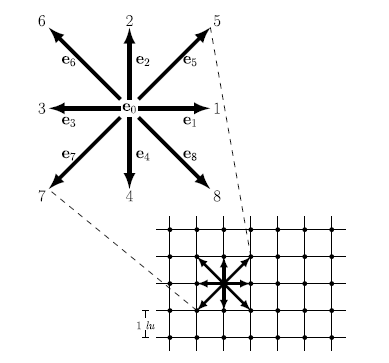
\includegraphics[scale=0.7]{Figures/d2q9.png}
    \caption{Malla D2Q9}
    \label{fig:14}
\end{figure}
donde $e = $ \textit{lu}\(/\)\textit{ts}. 
Usando el operador Bhatnagar–Gross–Krook para las colisiones del sistema, la ecuación del método queda de la siguiente forma \cite{bgk}:

\begin{align}
    f_\alpha(x + e_\alpha\Delta t, t + \Delta t) - f_\alpha(x,t) = -\frac{1}{\tau}[f_\alpha(x,t) - f^{(eq)}(x,t)] + S_\alpha(x,t)
\end{align}

donde $x = (x, y)$, \(\tau\) es el tiempo de relajación, \(f_\alpha\) es la función de distribución, $f_\alpha^{(eq)}$ es la función de distribución de equilibrio y \(S_\alpha(x,t)\) representa el termino de fuente, el cual se define de la siguiente manera:

\begin{align}
    S_\alpha = 
     \begin{cases}
       0 & \alpha = 0\\
       \dfrac{\Delta t}{6e^2}e_{\alpha i}F_i(x,t) - w_\alpha\dfrac{g\overline{h}(x,t)}{e^2}[b(x + e_\alpha\Delta t) - b(x)], & \alpha = 1,\dots,8 \\
     \end{cases}
\end{align} 

el cual incluye diferentes términos en su definición, tales como fuerzas superficiales, fuerzas volumétricas y el efecto \textit{bed slope}. 

A partir de la formula (5) y los aspectos mencionados en el Capítulo~\hyperref[sec:3.2]{3.2} es que se debe implementar LBM para programación paralela en GPU, principalmente pensando en el diseño de los elementos de las funciones de distribución (9 por cada ``nodo'') y que para poder calcular cada macro componente (fuerzas en cada eje y altura de la superficie del liquido) se necesitan elementos de las fuerzas de nodos adyacentes, por lo que se necesitaría una gestión adecuada de recursos en memoria.

Para la posterior experimentación, se utilizarán dos códigos generados por Álvaro Salinas, M.Sc., para su tesis titulada \textit{A high performance GPU implementation of the Lattice Boltzmann Method with open boundary conditions for solving the Shallow Water Equations in real scenarios}, cuya redacción fue para optar al grado de magíster en ciencias de la ingeniería informática en la Universidad Técnica Federico Santa María \cite{thesisB}.
Las implementaciones fueron, un framework general para futuros trabajos con distintas aplicaciones y funciones de equilibrio posibles, y una versión optimizada para la aplicación de las \textit{Shallow Water Equations} y condiciones de borde trabajadas en el paper \textit{Well-balanced open boundary condition in a lattice Boltzmann model for shallow water with arbitrary bathymetry} \cite{paperB}. 

Con tal de evitar cualquier tipo de error es que se planteó para ambas un \textit{Pull Scheme}, el cual consiste en utilizar 2 arreglos de memoria global en GPU para almacenar los 9 elementos de distribución de fuerzas de cada nodo con tal de reservar uno para lectura y otro para escritura respectivamente en cada \textit{time step}.
También, el diseño de estos se esquematiza de tal manera que exista un acceso coalescente a los arreglos, lo cual se logra posicionando de forma contigua aquellos elementos que se necesitan en una misma sección del kernel.
Esto fue nombrado como \textit{Struct of Arrays (SoA)} o arreglo de estructuras, mientras que una diseño no coalescente sería una estructura de arreglos o \textit{Array of Structs (AoS)} (ver Figura~\ref{fig:15}).

\begin{figure}[h!]
\centering
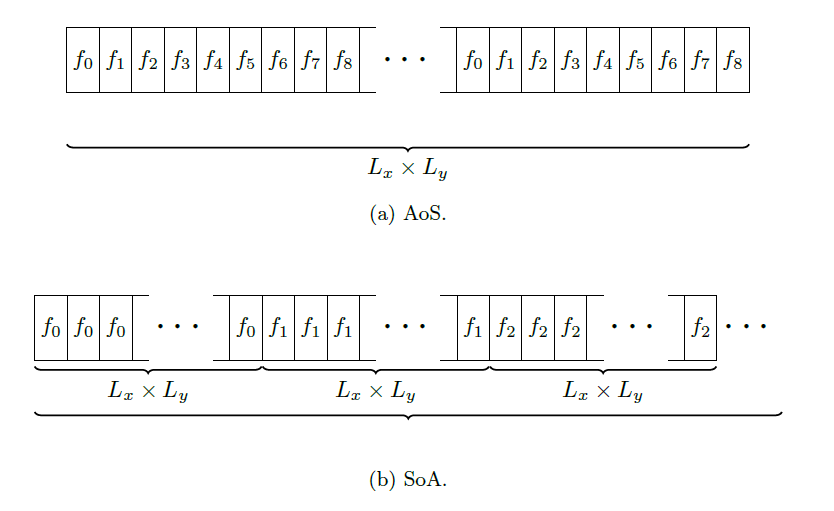
\includegraphics[width=0.6\textwidth]{Figures/layouts.png}
\caption{Diagrama de una Estructura de Arreglos \textit{(SoA)} y un Arreglo de Estructuras \textit{(AoS)}, fuente: \cite{thesisB}.}
\label{fig:15}
\end{figure}

\newpage


Para conseguir nuevos resultados y contrastar con los experimentos a realizar sobre los códigos de multiplicación de matrices, es que de todas formas se ejecutará una variación del código original del \textit{framework} con tal de no utilizar un acceso coalescente a la memoria y así analizar su efecto tanto en el tiempo de computo general como por cada sección del kernel de \textit{Pull Scheme}, cuya estructura general se presenta en el Algoritmo~\ref{alg:7}.

\begin{algorithm}
\caption{Kernel - \textit{Pull Scheme} en LBM}
\label{alg:7}
\begin{algorithmic}[1]
%\algsetup{linenosize=<size>}
\Procedure{TimeStep}{} %\(f_1\), \(f_2\), \(h\), \(b\), \(e\), \(Lx\), \(Ly\)
\If{se trabaja dentro del dominio de tamaño $Lx\times Ly$}
    \State definir \(f_\text{local}\)
    \For{fuerza $\alpha = [0,8]$}
        \If{necesita condición de borde abierta}
            \State \(f_\text{local}[\alpha]\) = \(f1[\alpha]\)
        \Else
            \State calcular S(\(\alpha\), \(h\), \(b\), \(e\))
            \State \(f_\text{local}[\alpha]\) = \(f1[\text{vecindario}][\alpha]\) + S
        \EndIf
    \EndFor
    \For{fuerza $\alpha = [0,8]$}
        \If{necesita condición de rebote \textit{Bounce Back}}
            \If{$\alpha \in {1,3,5,7}$}
                \State \(f_\text{local}[\alpha]\) = $f_\text{local}[\alpha + 2]$
            \Else
                \State \(f_\text{local}[\alpha]\) = $f_\text{local}[\alpha - 2]$
            \EndIf
        \EndIf
    \EndFor
    \State calcular variables macroscópicas \(h\), \(u\), \(v\)
    \For{fuerza $\alpha = [0,8]$}
        \State recalcular $f^{(eq)}$ = EDF(\(\alpha\), \(h\), \(u\), \(v\), \(e\))
        \State calcular y definir \(f_2[\alpha]\)
    \EndFor
\EndIf
\EndProcedure
\end{algorithmic}
\end{algorithm}

Con tal de obtener dicha comparativa, el código del kernel principal de \textit{LBM Framework} se subdividirá en los siguientes 3 kernels:

\begin{itemize}
    \item \verb|sourceForcing()|, en el que se hará el calculo parcial de las componentes de la función de distribución \(f_\alpha\) y aplicarán las condiciones de borden configuradas. Lineas 3 a 15 del Algoritmo~\ref{alg:7}.
    \item \verb|varMacroscopica|, en donde se recalcularán las variables macroscopicas. Linea 16 del Algoritmo~\ref{alg:7}.
    \item \verb|fUpdate()|, en el que se recalcularán los elementos de la función de equilibrio para el \textit{time step} actual y se recalculará \(f\). Linea 17 del Algoritmo~\ref{alg:7}.
\end{itemize}
\newpage
\secnumbersection{Ejecución de códigos y análisis de resultados.}
\hlabel{sec:4}

El primer resultado a analizar corresponde a la ejecución del kernel {\verb vectorAdd() } propuesto en el capitulo 3, en ambas tarjetas gráficas utilizadas definiendo un tamaño de vector en aumento.
Los tamaños de vectores utilizado corresponden a una sucesión geométrica definida por la formula,
\begin{equation*}
    M = 2^i , i \in [8,9,\dots,29,30]
\end{equation*}
En la Figura~\ref{fig:16} se presenta el gráfico de tiempo de ejecución (en milisegundos) versus el tamaño del vector.
En este, se puede observar como en las primeras instancias el tiempo de ejecución de la tarjeta de AMD es mucho mayor a la de la tarjeta de NVIDIA.
Sin embargo, para instancias más grandes el tiempo de ejecución se ve disminuido significativamente.
Por otro lado, se nota que la tarjeta de AMD logra ejecutar 2 instancias más para $i = 28$ e $i = 29$, lo cual va de acuerdo a las especificaciones de ambas tarjetas definidas en el capitulo 3.1, presentando una mayor memoria la GPU de AMD.
Esta conclusión se obtiene a partir de la formula de tamaño de memoria teórico de un vector, definido por
\begin{equation}
    m = n \times s
\end{equation}
%$$  s $$
en donde \(m\) corresponde al tamaño total del arreglo en bytes, \(n\) al tamaño del arreglo y \(s\) al tamaño en bytes del elemento utilizado ( 4 en el caso del tipo de dato \textit{float}).
Respecto a la formula anterior, hay que destacar que esta no puede ''igualarse'' a la cantidad de memoria total de la GPU ya que esta también es utilizada por el sistema operativo  para poder renderizar la interfaz de una computadora en al menos aquellas que la utilicen. 

Por último, en lo que concierne a la diferencia de rendimiento en las primeras instancias del gráfico, el principal factor al que se le puede atribuir es a la función de lanzamiento de kernel definido por ROCm ({\verb hipLaunchKernelGGL() }), ya que el otro factor del que podría depender es la inicialización de vectores, pero esto no es considerado en el tiempo de computo de los kernel.

\begin{figure}[h!]
\centering
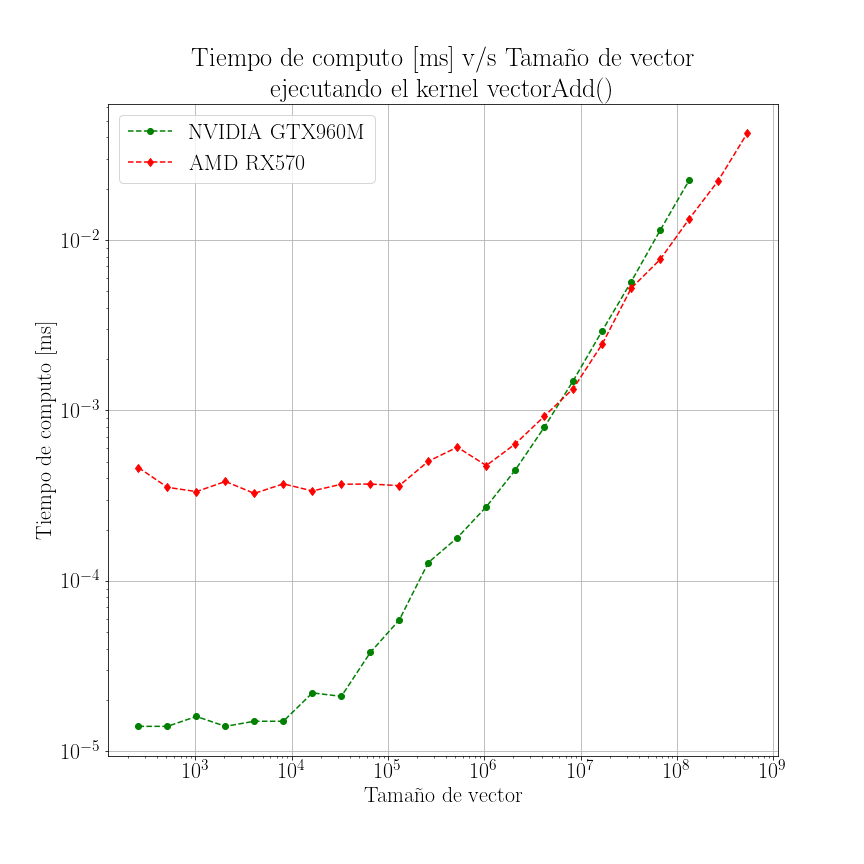
\includegraphics[width=0.8\textwidth]{Figures/plot1.png}
\caption{Gráfico de tiempo de computo versus tamaño de vector al ejecutar el kernel  vectorAdd() .}
\label{fig:16}
\end{figure}

\newpage

%-----------------------------------------------------

El segundo conjunto de resultados, corresponde a la ejecución del kernel {\verb  matrixMul()} en sus cuatro versiones para uso en GPU y explicadas en el Capítulo~\hyperref[sec:3.2]{3.2}, estándar, aplicando \textit{Tiling}, accediendo de forma coalescente en la memoria global y utilizando el producto externo.
Los gráficos de la Figura~\ref{fig:17} corresponden a los resultados (en términos de tiempo de computo y rendimiento) de las distintas versiones de {\verb matrixMul() } antes mencionadas, en ambas tarjetas y para multiplicación de matrices de tamaño \(10240\times10240\), las cuales de acuerdo a la formula 7 utilizan $10240\times10240\times4~\text{[byte]} \approx 419~\text{[Mbyte]}$.
De acuerdo a los resultados, en dos de las tres optimizaciones se observa una mejora significativa respecto a versiones anteriores.
Sin embargo, el acceso coalescente a la memoria global de la matriz de \(B\) provoca en resultados mucho peores que incluso la versión estándar.
Dicho comportamiento puede deberse a un \textit{trade off} entre utilizar un acceso coalescente a la memoria global de \(B\) versus un cambio de forma en el acceso a la memoria compartida, mejor conocido como \textit{Bank Conflict}.
Este termino viene en que, para aumentar el ancho de banda efectivo al realizar accesos a memoria compartida, los datos de esta están divididos en diferentes módulos (o \textit{Banks}).
Así, si múltiples \textit{threads} deben hacer accesos a diferentes \textit{Banks} estos serán simultáneos, mientras que si se deben realizar accesos a un mismo \textit{Bank}, estos se harán de forma secuencial \cite{bank}.

Otra diferencia encontrada es que en la versión de acceso coalescente a memoria global, el resultado de NVIDIA es peor tanto en Gflop/s como en tiempo de ejecución respecto de la versión estándar, mientras que en AMD el resultado sigue siendo un poco mejor.
Esto puede deberse a un manejo optimizado en el acceso a memorias por parte de los controladores de AMD, evidenciando así mismo un mejor rendimiento general para dicho volumen de datos (dejando de lado las especificaciones generales). 

\begin{figure}[H]
  \centering
  \begin{subfigure}{0.5\textwidth}
    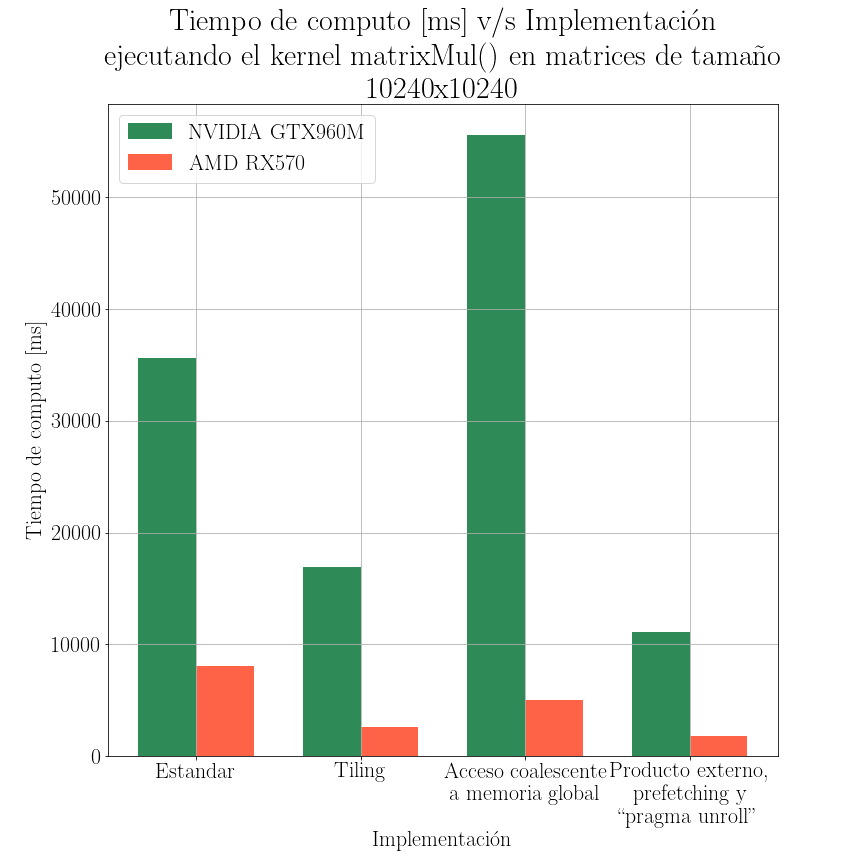
\includegraphics[width=\linewidth]{Figures/plot2.png}
    \caption{} 
  \end{subfigure}%
  \begin{subfigure}{0.5\textwidth}
    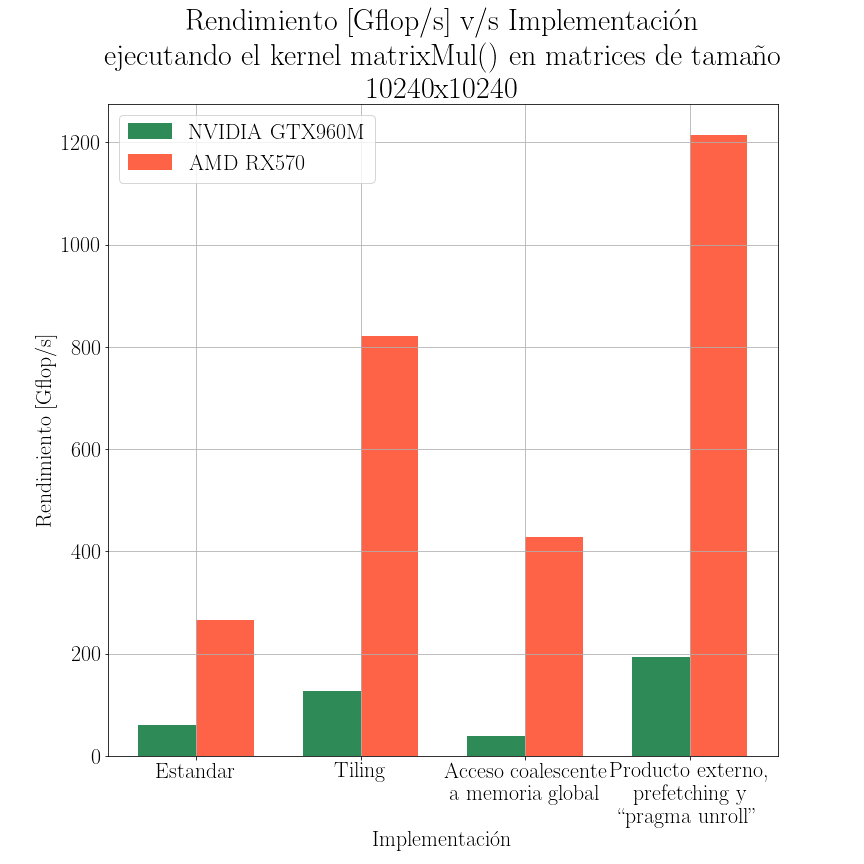
\includegraphics[width=\linewidth]{Figures/plot3.png}
    \caption{} 
  \end{subfigure}%
  \caption{Gráfico de tiempo de computo y rendimiento versus tamaño de vector al ejecutar el kernel matrixMul().}
  \label{fig:17}
\end{figure}

%------------------------

\newpage

Los resultados de la experimentación realizada sobre la implementación optimizada del método de Lattice Boltzmann se presentan en la Figura~\ref{fig:18}.
En dicha gráfica, se presentan los tiempos de ejecución por 20000 \textit{time steps} de 3 segundos reales cada uno, del código optimizado con 5 instancias (archivos) de entrada:

\begin{itemize}
    \item Iquique, correspondiente a niveles de agua de un tsunami registrado el año 2014 en la misma localidad, como grilla de \(549\times821\) nodos.
    \item Maule, correspondiente a niveles de agua de un tsunami registrado el año 2010 en la misma localidad, como grilla de \(158\times241\) nodos.
    \item Talinay, correspondiente a un datos de un tsunami ocurrido en la misma localidad, como grilla de \(124\times241\) nodos.
    \item Test40000, instancia de ejemplo del repositorio de LBM optimizado, de tamaño \(200\times200\) nodos.
    \item Test4000000, una instancia generada a partir de una función 
    \begin{equation*}
        f(x,y) = 5\exp\,\left(-50(0.013y^2 + 0.08125(x+0.5)^2)\right) + 1199
    \end{equation*}
    con $x,y \in [-2,2]\times[-2,2]$ en la que el dominio posee una ``costa'' para cada $x > 0.5$ de tamaño \(2000\times2000\) nodos.
\end{itemize}

En general, los resultados de ambas tarjetas gráficas siguen un mismo patrón en comparación a la magnitud del volumen de información entregado por los archivos de entrada para un mismo número de pasos del método de Lattice Boltzmann.
Los archivos de salida de las versiones del código para AMD y NVIDIA producen los mismos archivos, cuyos gráficos de calor se presentan en las 
% Figuras~\ref{fig:20},\ref{fig:21},\ref{fig:22},\ref{fig:23},\ref{fig:24}.
Figuras~\ref{fig:20}-\ref{fig:24}.
El rango del mapa de calor de las imágenes se define en base a la media de los niveles de agua presenten en todos los archivos de salida a graficar.

\begin{figure}[H]
  \centering
    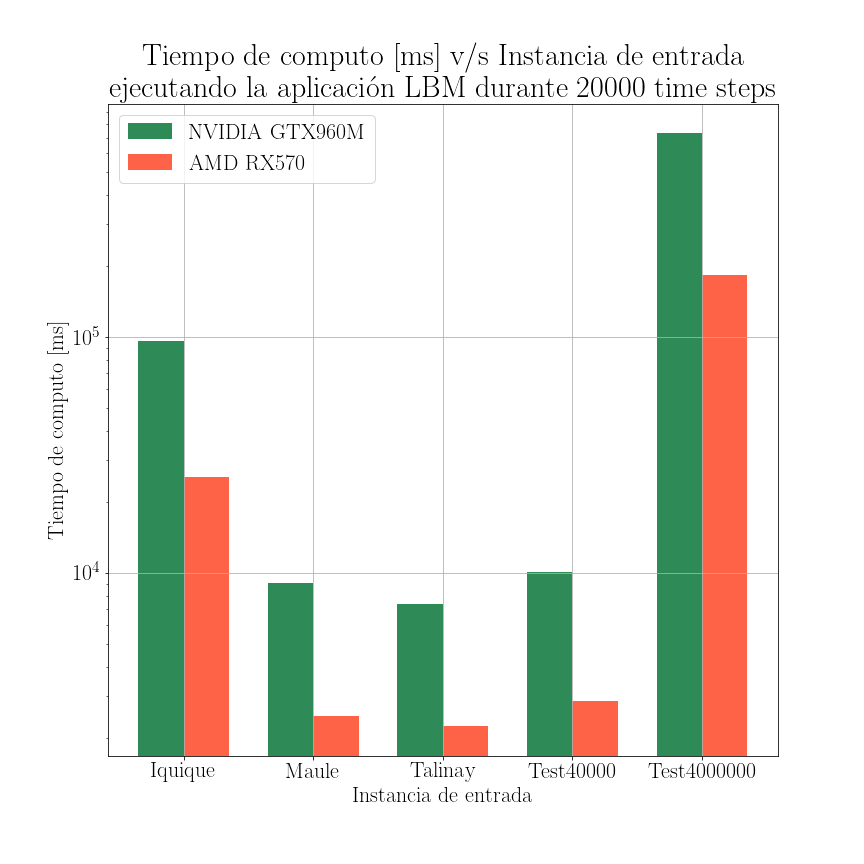
\includegraphics[width=0.8\linewidth]{Figures/plot4.png}
  \caption{Gráfico de tiempo de computo versus archivo de entrada al ejecutar el código optimizado de LBM por 20000 \textit{time steps}.}
  \label{fig:18}
\end{figure}

Los resultados de tiempos de computo por cada ``sub kernel'' generado sobre el kernel original del código \textit{LBM Framework} se presentan en los gráfico de la Figura~\ref{fig:19-1} y \ref{fig:19-2}, para CUDA y ROCm.
Se ejecutaron 10000 \textit{time steps} de archivos de entrada, representando instancias de nodos cuadrada, en donde un aumento en el tamaño del lado de forma exponencial es la única diferencia entre los archivos.
La situación simulada, esta compuesta por una superficie de agua modelada por la función
\begin{equation*}
    0.1\exp\left(-50(x^2 + y^2)\right) + 50
\end{equation*}
con $x,y \in [-4,4]\times[-4,4]$
Además, no se aplicaron condiciones de borde extra además de aquellas presentes en los bordes de la grilla.

A partir de lo que se observa, se puede notar que tan solo existen diferencias significativas en el primer y tercer kernels a lo largo de todos las ejecuciones de ambos diseños de arreglos \(f_1\) y \(f_2\).
Esto se debe a que en el segundo kernel no hay accesos al arreglo \(f_1\) o \(f_2\).
Esto implica que, en la ejecución de un framework generalizado no afecta de manera significativa el acceso coalescente a la memoria, por lo menos al hacer uso de GPU's de venta en mercado general (computadoras personales).
Sin embargo, se debe recalcar que al momento de ejecutar un software de este tipo con inputs de volumen mucho mayor, la diferencia de tiempo presente se hace cada vez notable, por lo que esta si debiera ser significativa al utilizar clústers de nodos de procesamiento o supercomputadoras con GPU's de características de gran magnitud.


\begin{figure}[H]
  \centering
  \begin{subfigure}{0.5\textwidth}
    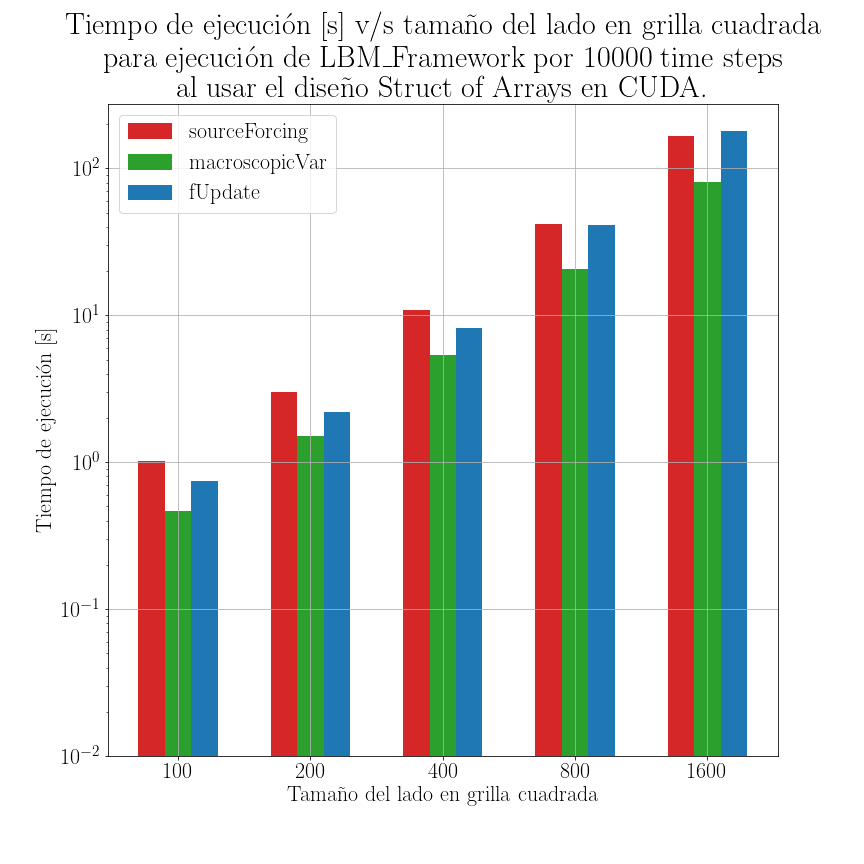
\includegraphics[width=\linewidth]{Figures/plot6.png}
    \caption{} 
  \end{subfigure}%
  \begin{subfigure}{0.5\textwidth}
    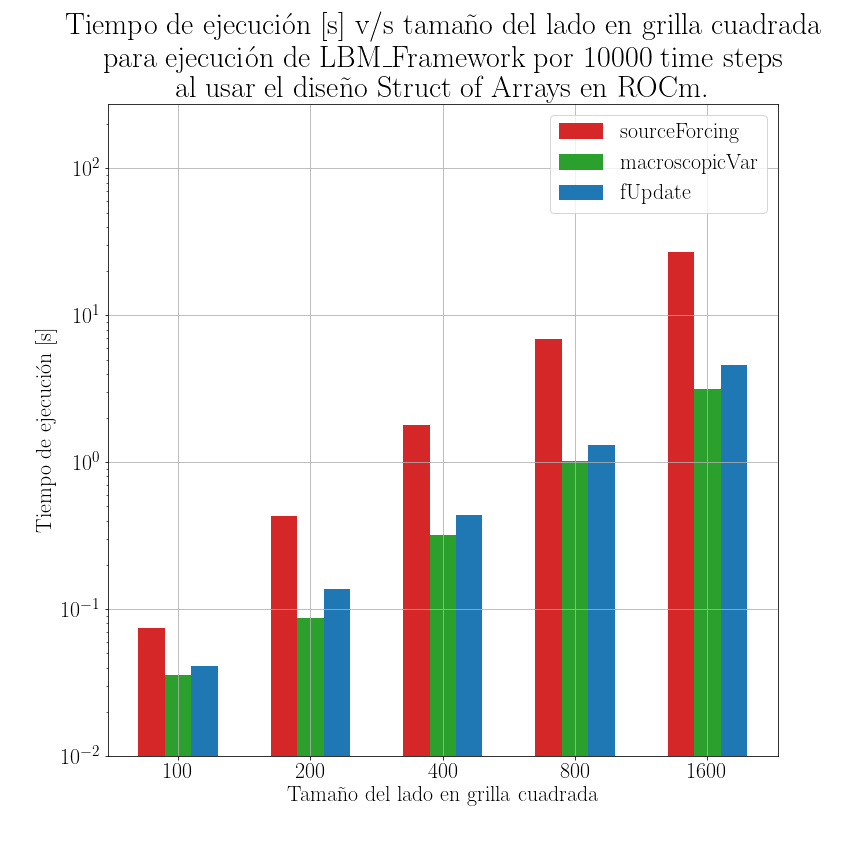
\includegraphics[width=\linewidth]{Figures/plot8.png}
    \caption{} 
  \end{subfigure}%
  \caption{Gráfico de tiempo de cómputo versus tamaño de archivo input ejecutando el código \textit{LBM Framework} por 10000 \textit{time steps} usando SoA y AoS en el diseño de los arreglos \(f_1\) y \(f_2\) en CUDA.}
  \label{fig:19-1}
\end{figure}

\begin{figure}[H]
  \centering
  \begin{subfigure}{0.5\textwidth}
    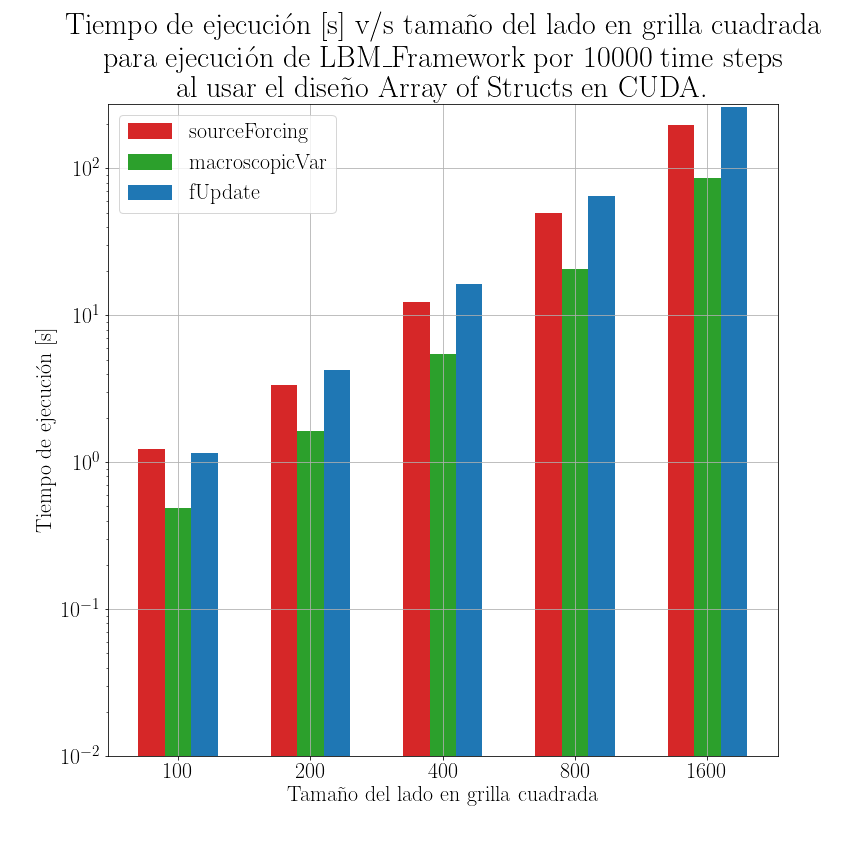
\includegraphics[width=\linewidth]{Figures/plot7.png}
    \caption{} 
  \end{subfigure}%
  \begin{subfigure}{0.5\textwidth}
    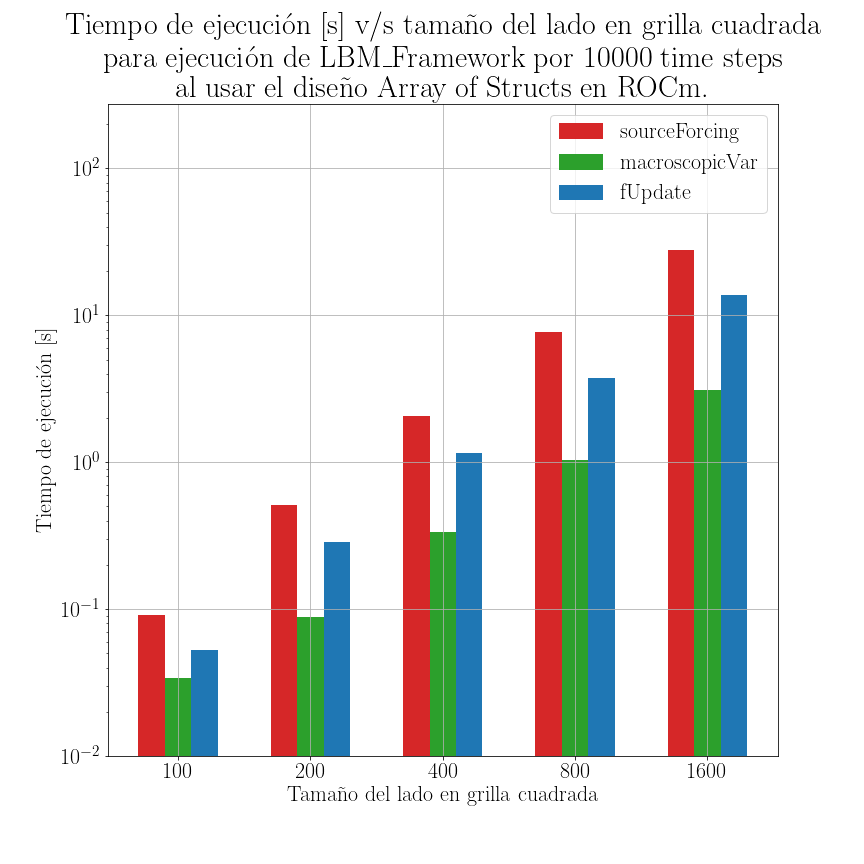
\includegraphics[width=\linewidth]{Figures/plot9.png}
    \caption{} 
  \end{subfigure}%
  \caption{Gráfico de tiempo de cómputo versus tamaño de archivo input ejecutando el código \textit{LBM Framework} por 10000 \textit{time steps} usando SoA y AoS en el diseño de los arreglos \(f_1\) y \(f_2\) en ROCm.}
  \label{fig:19-2}
\end{figure}

%

Con tal de cumplir el objetivo que buscaba proponer instancias de posibles tsunamis en costas Chilenas, es que se presentan las 
Figuras~\ref{fig:25}-\ref{fig:27}.
Estas situaciones corresponden a niveles de agua generados a partir de funciones similares a las de instancias anteriores, correspondientes a:

\begin{itemize}
    \item \textbf{Antofagasta}, que simulan las costas de la ciudad de Antofagasta desde las latitudes 23°23'36.6"S a 24°03'40.7"S aproximadamente. 
    Los niveles de agua están modelados por la función
    \begin{equation*}
        f(x,y) = 5\,\exp\left(-50(0.08x^2 + 0.25(y+1)^2)\right) + 500
    \end{equation*}
    con \(x,y\in[-3,3]\times[-3,-3]\) y una rotación antihoraria de 30°.
    \item \textbf{Serena}, que simulan las costas de la ciudad de La Serena desde las latitudes 29°29'31.8"S a 30°27'32.6"S aproximadamente.
    Los niveles de agua están modelados por la función
    \begin{equation*}
        f(x,y) = 5\,\exp\left(-50(0.25x^2 + 0.25(y+1)^2)\right) + 500
    \end{equation*}
    con \(x,y\in[-3,3]\times[-3,-3]\).
    \item \textbf{Valparaiso}, que simulan el litoral central Chileno desde las latitudes 31°54'00.3"S a 34°20'33.8"S aproximadamente.
    Los niveles de agua están modelados por la función
    \begin{equation*}
        f(x,y) = 5\,\exp\left(-50(0.08x^2 + 0.005(y+1)^2)\right) + 500
    \end{equation*}
    con \(x,y\in[0,6]\times[-3,-3]\).
\end{itemize}

En estas simulaciones realizadas, cada \textit{time step} corresponde a 3 segundos reales.

%--------------------------------------------



\begin{figure}[H]
\centering
\begin{subfigure}[b]{.4\linewidth}
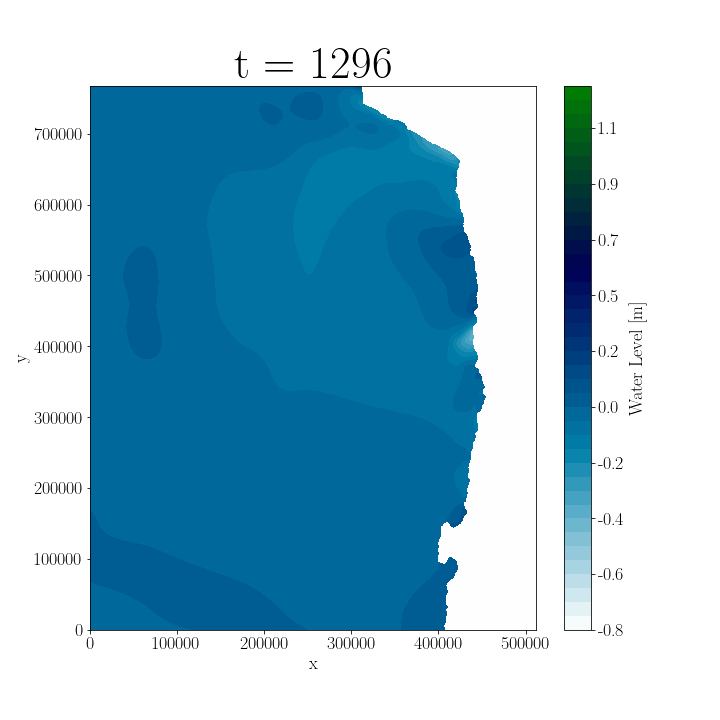
\includegraphics[width=\linewidth]{Figures/1-1.png}
\caption{}
\end{subfigure}
\begin{subfigure}[b]{.4\linewidth}
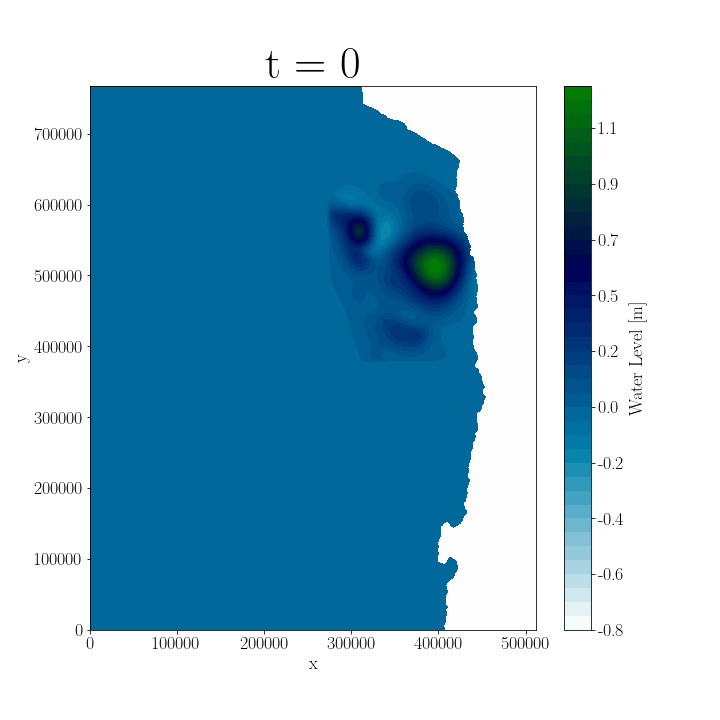
\includegraphics[width=\linewidth]{Figures/1-2.png}
\caption{}
\end{subfigure}

\begin{subfigure}[b]{.4\linewidth}
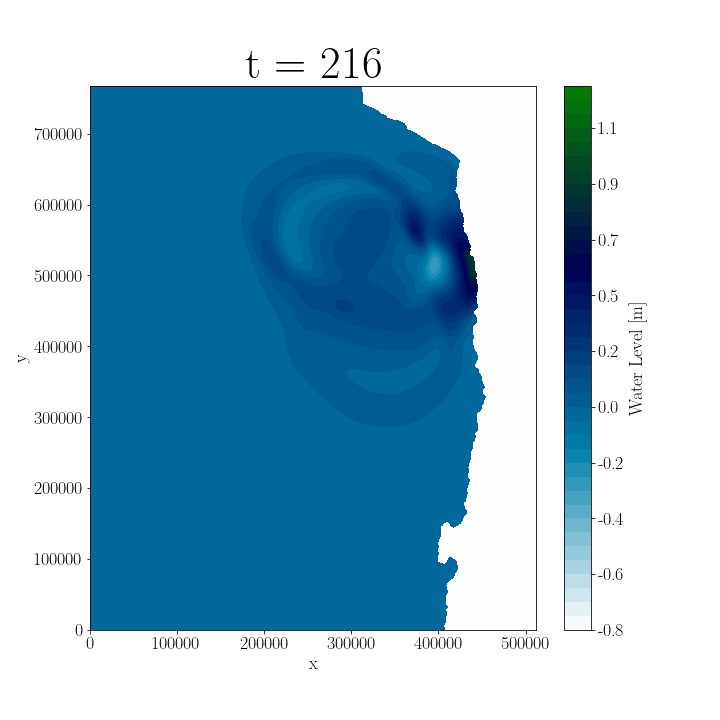
\includegraphics[width=\linewidth]{Figures/1-3.png}
\caption{}
\end{subfigure}
\begin{subfigure}[b]{.4\linewidth}
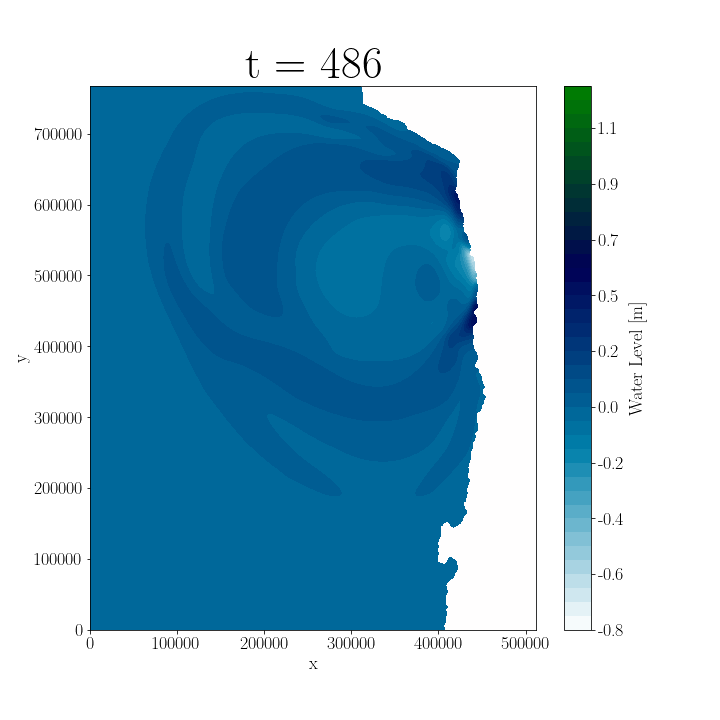
\includegraphics[width=\linewidth]{Figures/1-4.png}
\caption{}
\end{subfigure}

\begin{subfigure}[b]{.4\linewidth}
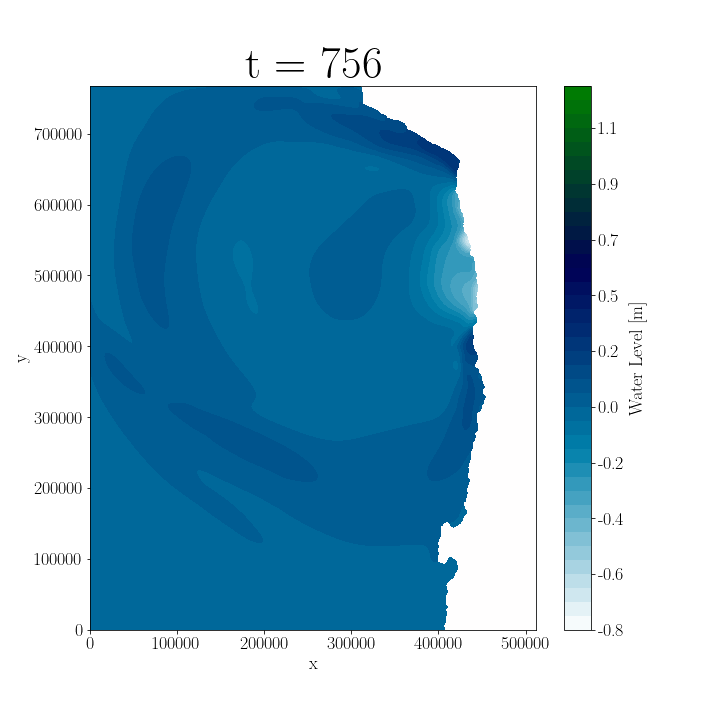
\includegraphics[width=\linewidth]{Figures/1-5.png}
\caption{}
\end{subfigure}
\begin{subfigure}[b]{.4\linewidth}
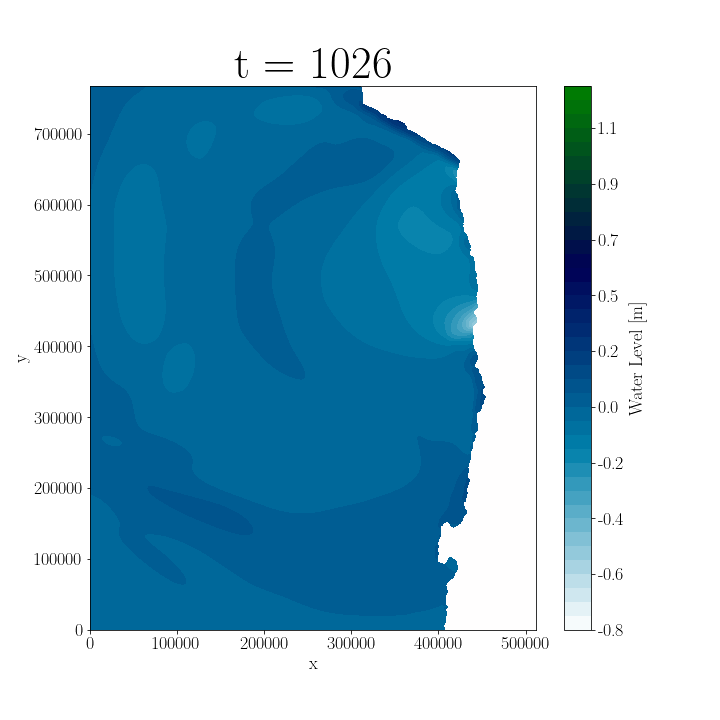
\includegraphics[width=\linewidth]{Figures/1-6.png}
\caption{}
\end{subfigure}


\caption{Niveles de agua de la salida de ejecutar el código de LBM optimizado con el archivo de entrada \textbf{Iquique}.}
\label{fig:20}
\end{figure}

%--------------------------------------------

\begin{figure}[H]
\centering
\begin{subfigure}[b]{.4\linewidth}
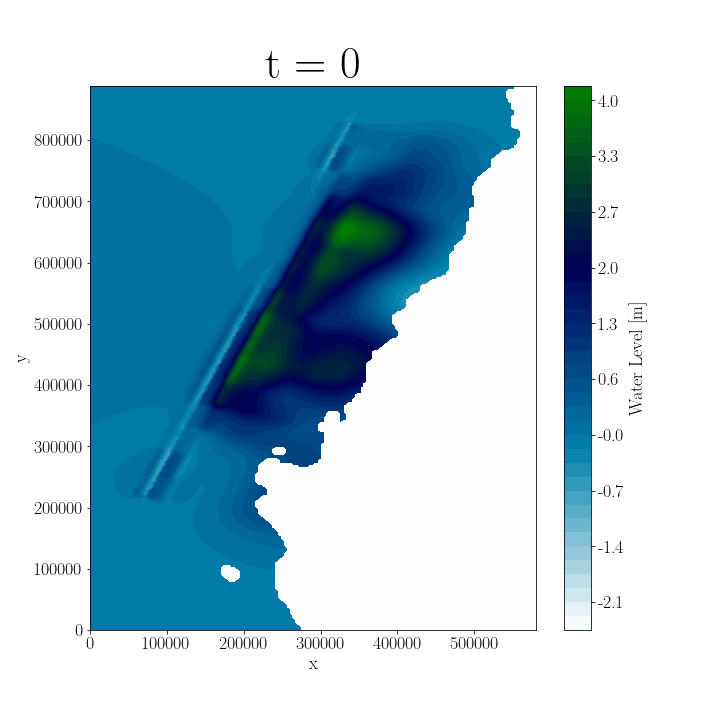
\includegraphics[width=\linewidth]{Figures/2-1.png}
\caption{}
\end{subfigure}
\begin{subfigure}[b]{.4\linewidth}
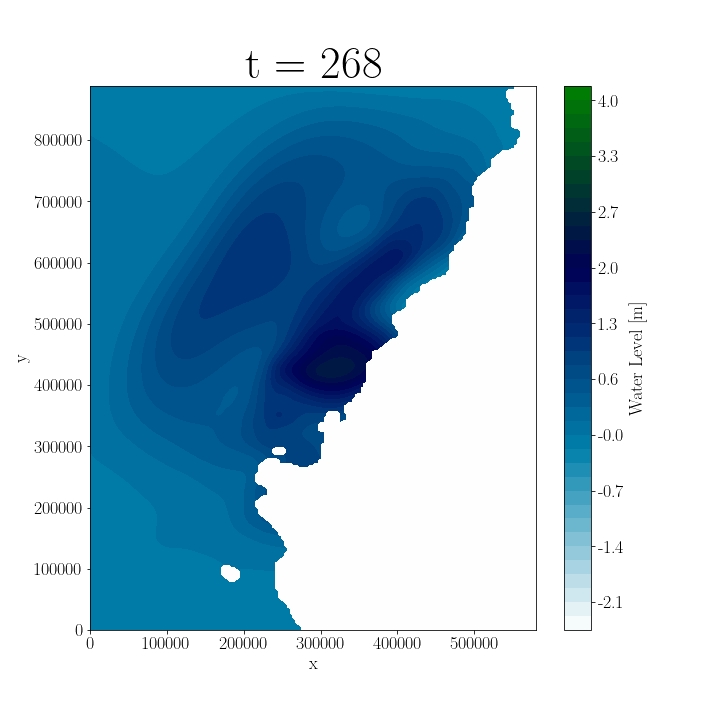
\includegraphics[width=\linewidth]{Figures/2-2.png}
\caption{}
\end{subfigure}

\begin{subfigure}[b]{.4\linewidth}
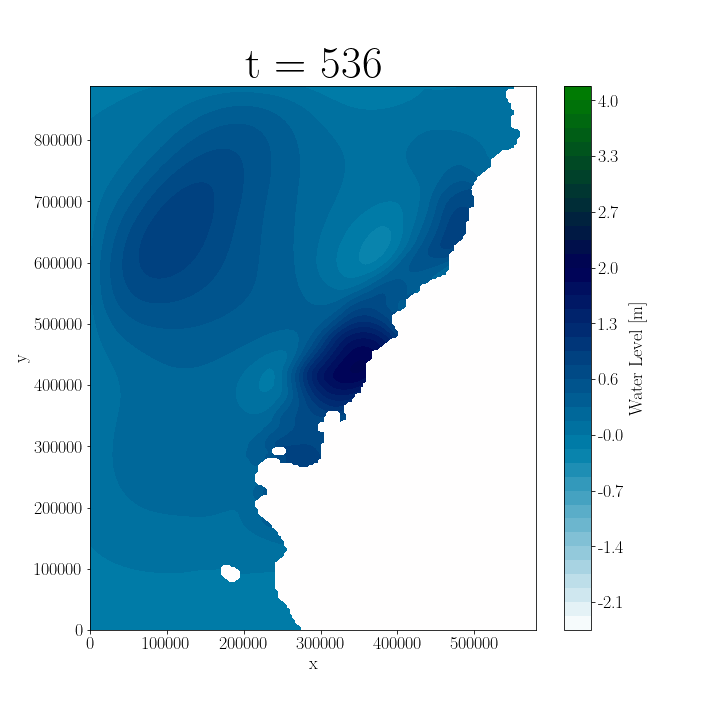
\includegraphics[width=\linewidth]{Figures/2-3.png}
\caption{}
\end{subfigure}
\begin{subfigure}[b]{.4\linewidth}
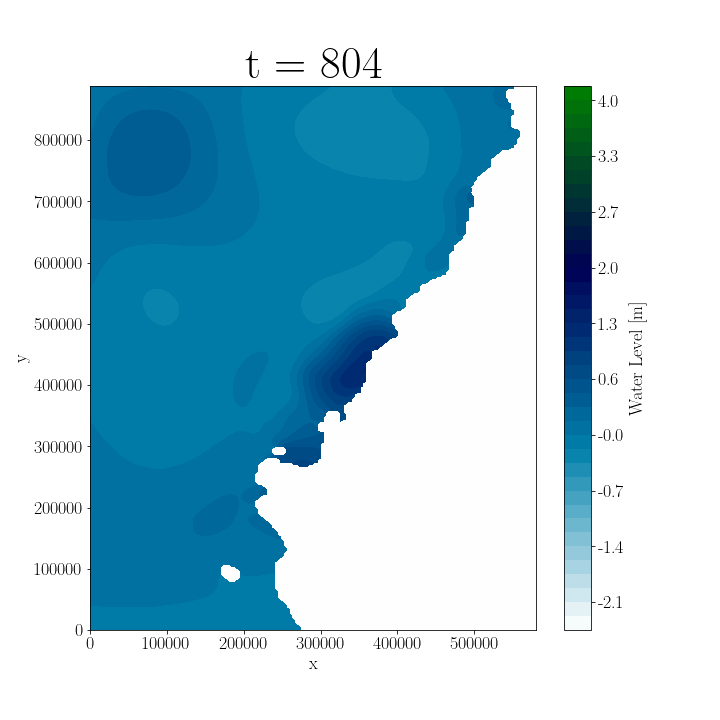
\includegraphics[width=\linewidth]{Figures/2-4.png}
\caption{}
\end{subfigure}

\begin{subfigure}[b]{.4\linewidth}
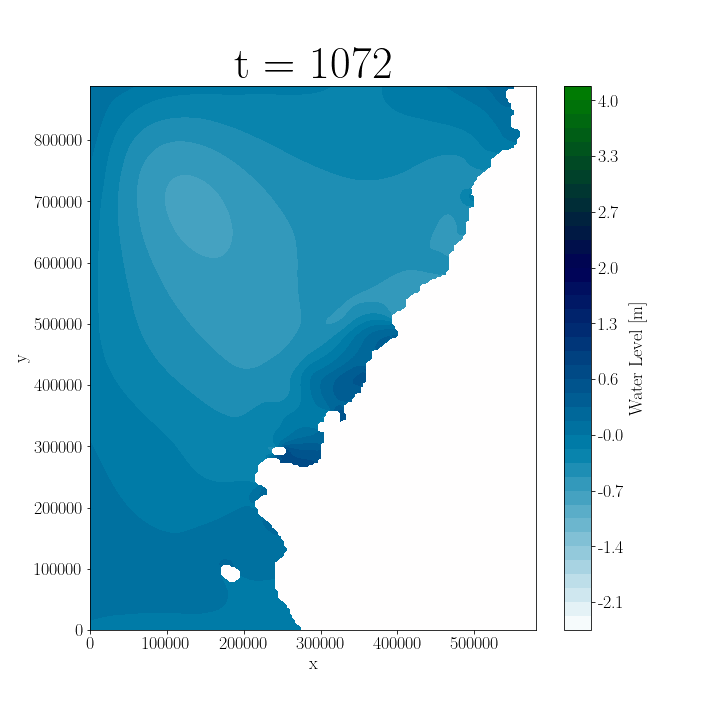
\includegraphics[width=\linewidth]{Figures/2-5.png}
\caption{}
\end{subfigure}
\begin{subfigure}[b]{.4\linewidth}
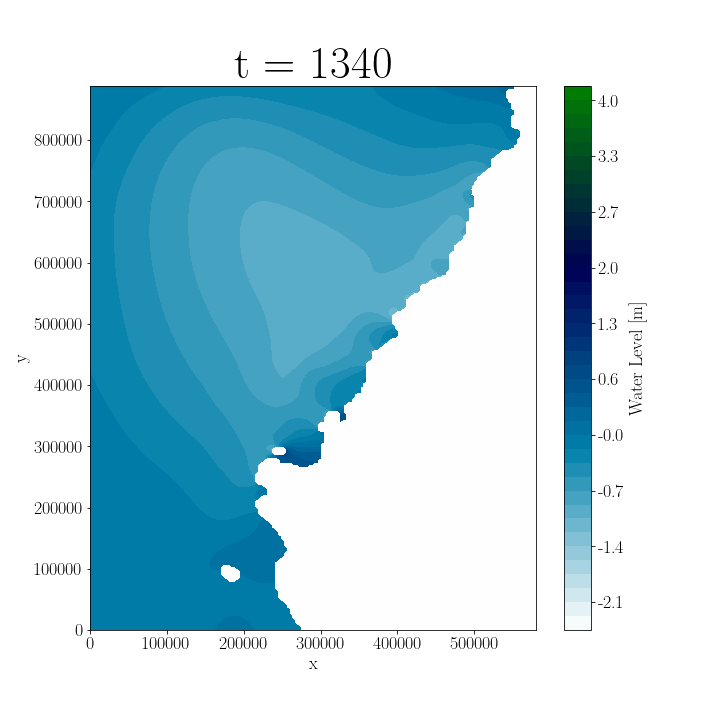
\includegraphics[width=\linewidth]{Figures/2-6.png}
\caption{}
\end{subfigure}
\caption{Niveles de agua de la salida de ejecutar el código de LBM optimizado con el archivo de entrada \textbf{Maule}.}
\label{fig:21}
\end{figure}

%--------------------------------------------

\begin{figure}[H]
\centering
\begin{subfigure}[b]{.4\linewidth}
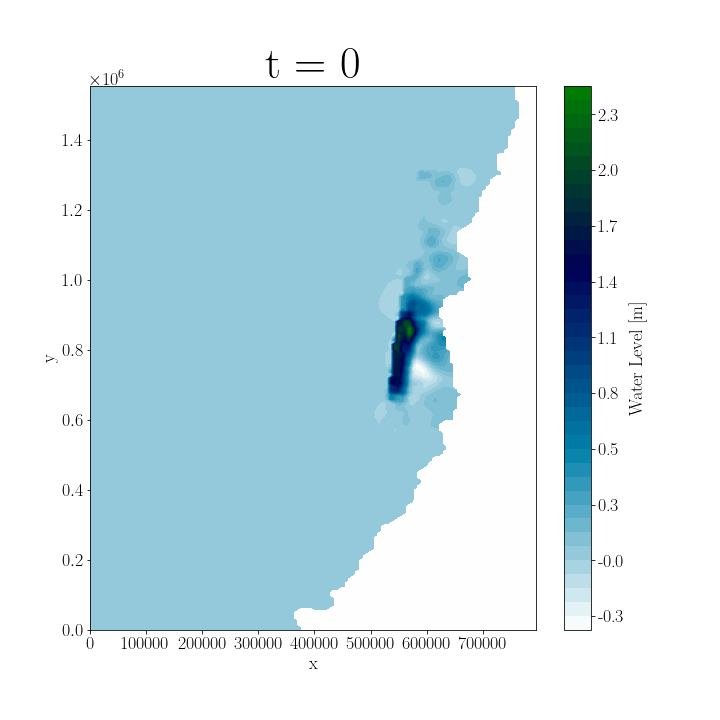
\includegraphics[width=\linewidth]{Figures/3-1.png}
\caption{}
\end{subfigure}
\begin{subfigure}[b]{.4\linewidth}
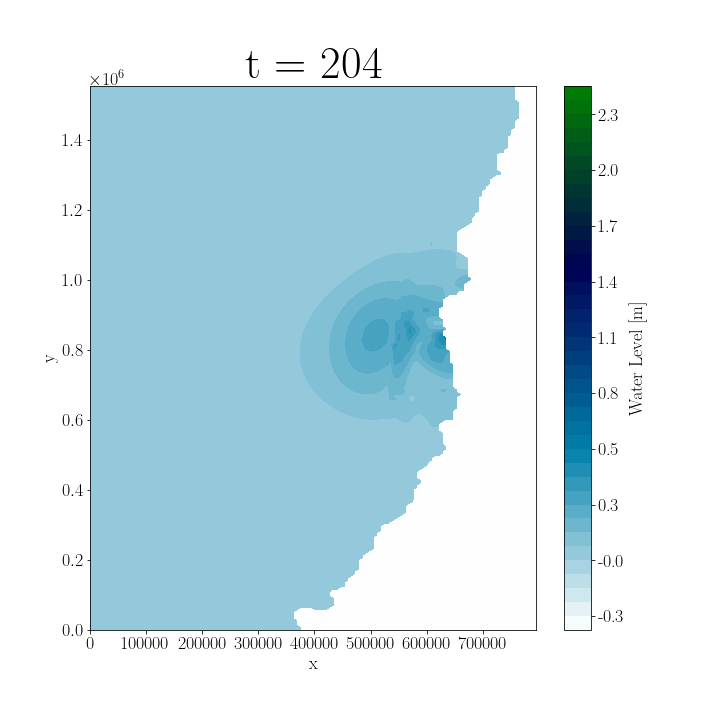
\includegraphics[width=\linewidth]{Figures/3-2.png}
\caption{}
\end{subfigure}

\begin{subfigure}[b]{.4\linewidth}
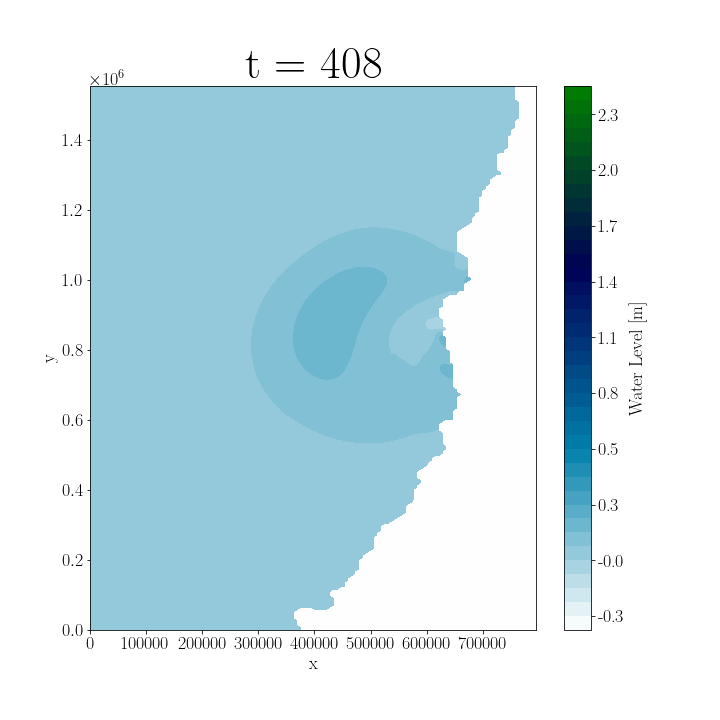
\includegraphics[width=\linewidth]{Figures/3-3.png}
\caption{}
\end{subfigure}
\begin{subfigure}[b]{.4\linewidth}
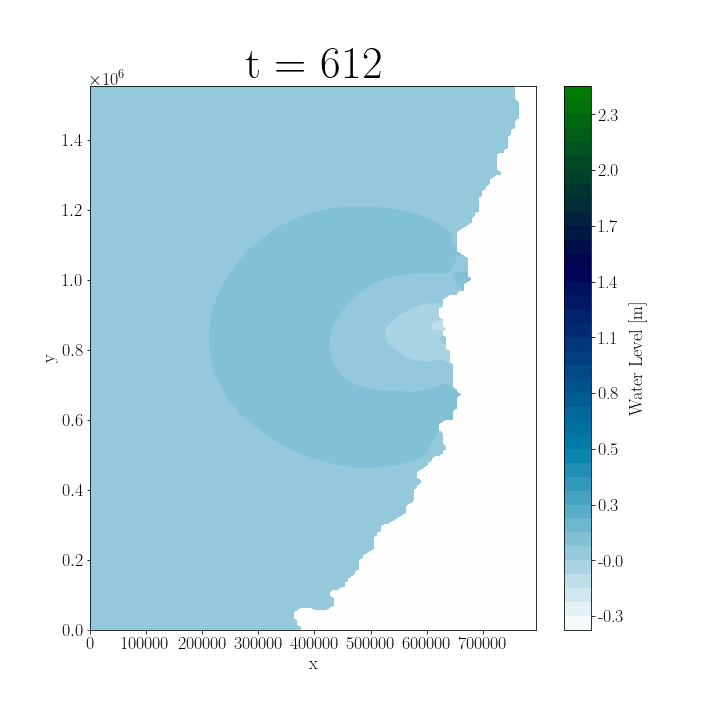
\includegraphics[width=\linewidth]{Figures/3-4.png}
\caption{}
\end{subfigure}

\begin{subfigure}[b]{.4\linewidth}
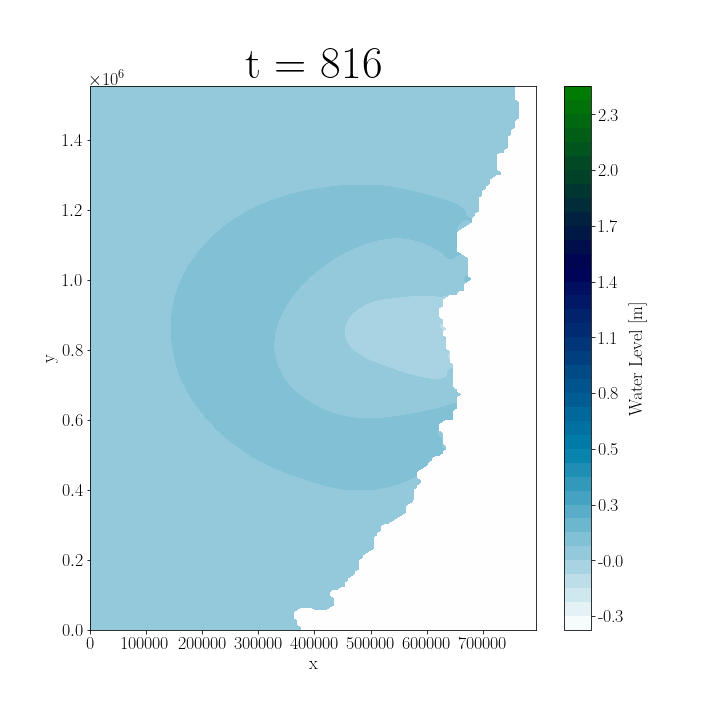
\includegraphics[width=\linewidth]{Figures/3-5.png}
\caption{}
\end{subfigure}
\begin{subfigure}[b]{.4\linewidth}
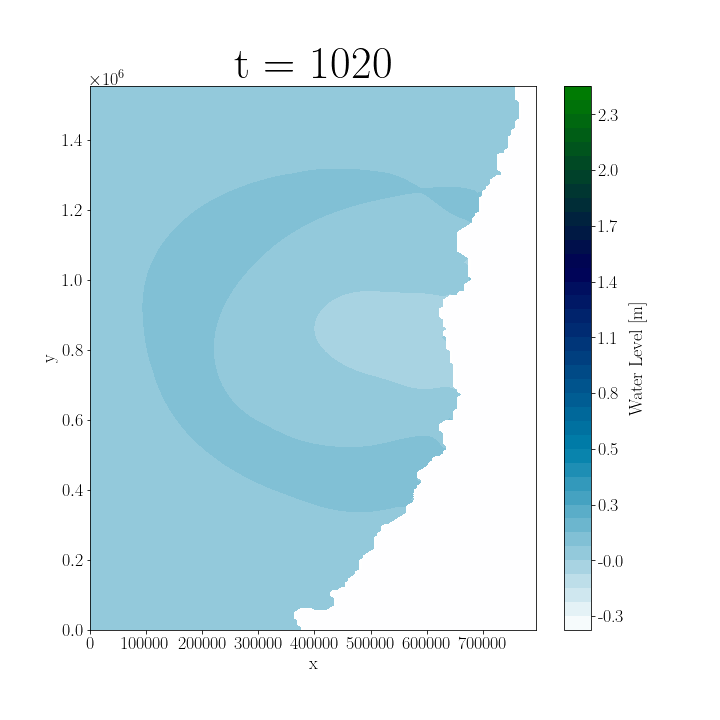
\includegraphics[width=\linewidth]{Figures/3-6.png}
\caption{}
\end{subfigure}
\caption{Niveles de agua de la salida de ejecutar el código de LBM optimizado con el archivo de entrada \textbf{Talinay}.}
\label{fig:22}
\end{figure}

%--------------------------------------------

\begin{figure}[H]
\centering
\begin{subfigure}[b]{.4\linewidth}
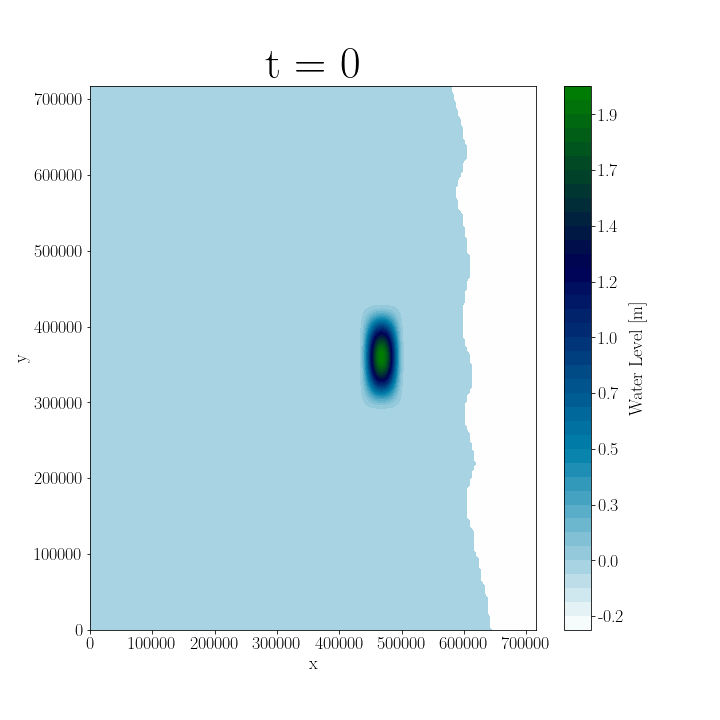
\includegraphics[width=\linewidth]{Figures/4-1.png}
\caption{}
\end{subfigure}
\begin{subfigure}[b]{.4\linewidth}
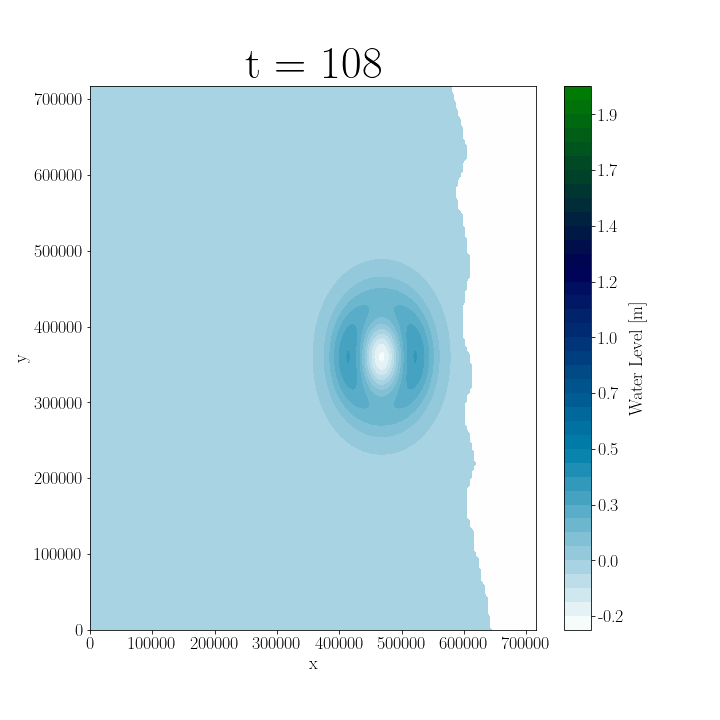
\includegraphics[width=\linewidth]{Figures/4-2.png}
\caption{}
\end{subfigure}

\begin{subfigure}[b]{.4\linewidth}
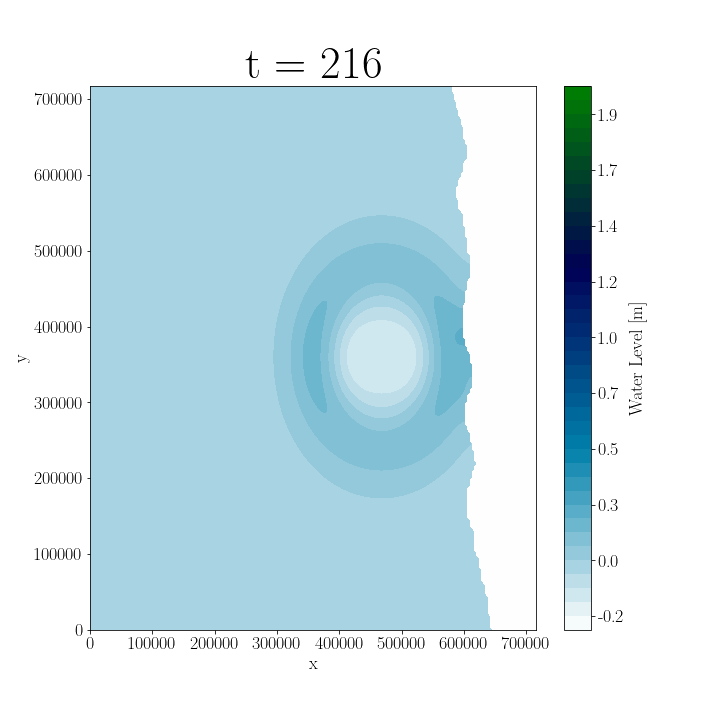
\includegraphics[width=\linewidth]{Figures/4-3.png}
\caption{}
\end{subfigure}
\begin{subfigure}[b]{.4\linewidth}
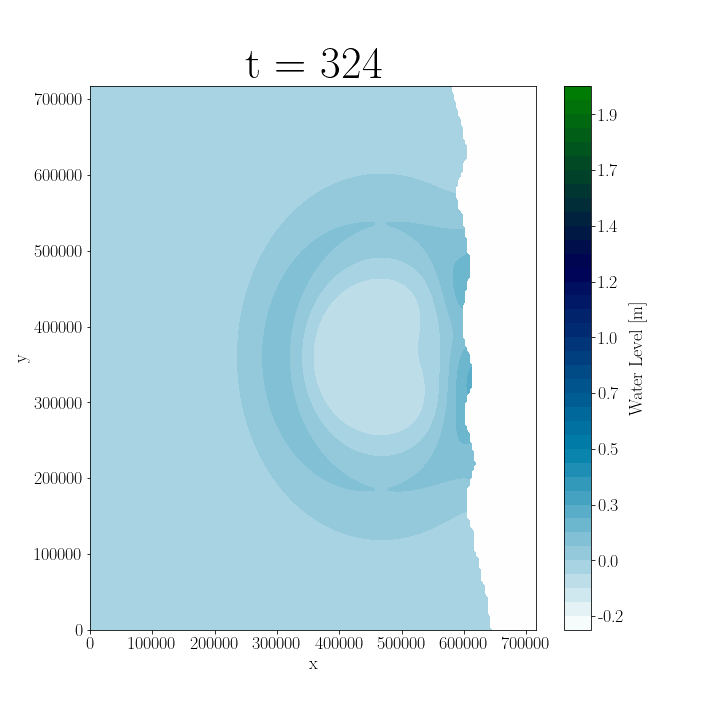
\includegraphics[width=\linewidth]{Figures/4-4.png}
\caption{}
\end{subfigure}

\begin{subfigure}[b]{.4\linewidth}
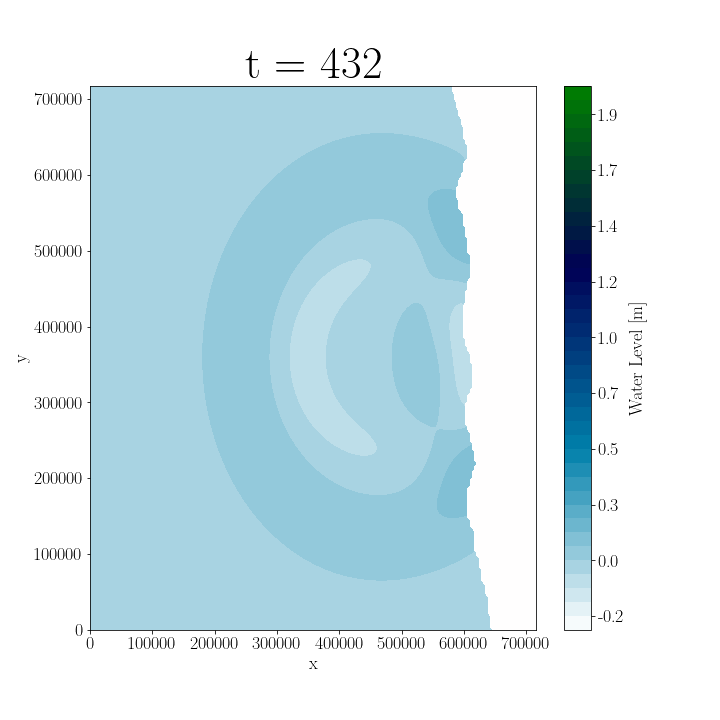
\includegraphics[width=\linewidth]{Figures/4-5.png}
\caption{}
\end{subfigure}
\begin{subfigure}[b]{.4\linewidth}
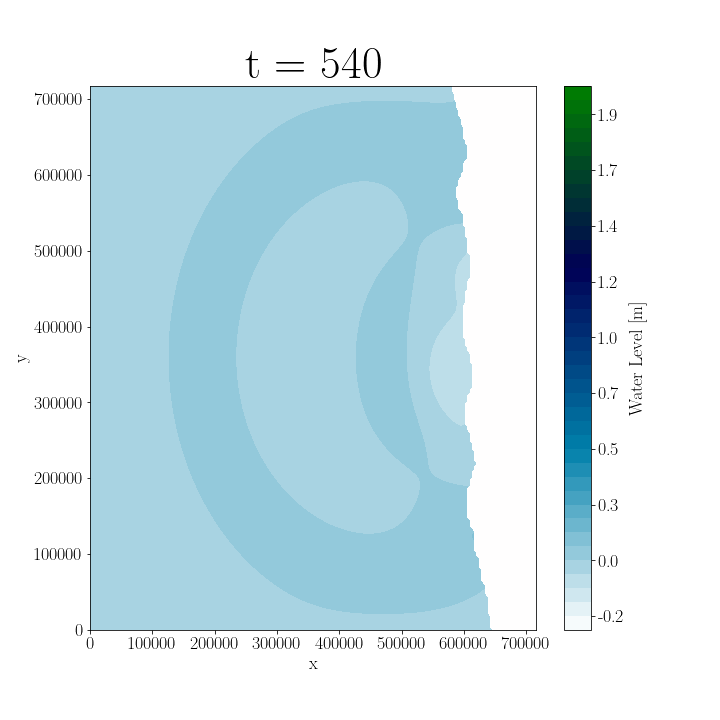
\includegraphics[width=\linewidth]{Figures/4-6.png}
\caption{}
\end{subfigure}

\caption{Niveles de agua de la salida de ejecutar el código de LBM optimizado con el archivo de entrada \textbf{Test40000}.}
\label{fig:23}
\end{figure}

%--------------------------------------------

\begin{figure}[H]
\centering
\begin{subfigure}[b]{.4\linewidth}
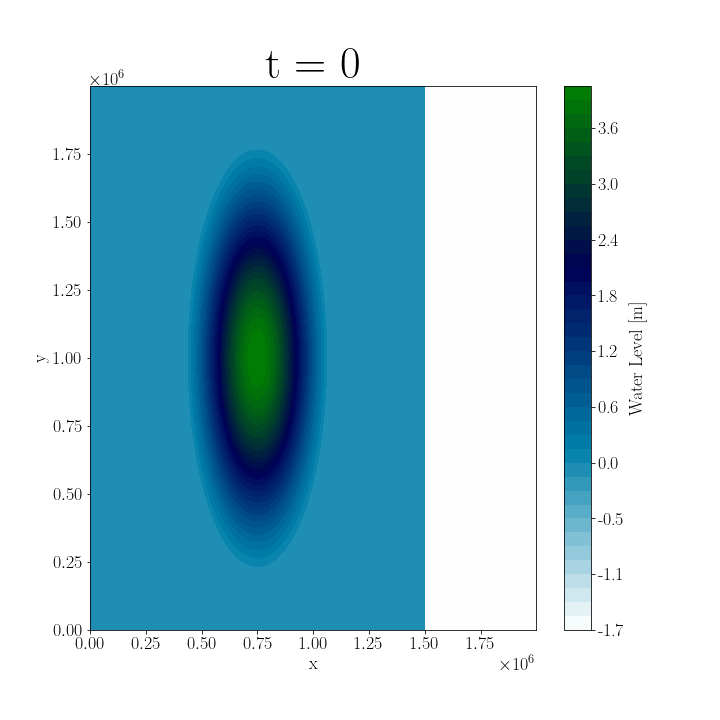
\includegraphics[width=\linewidth]{Figures/5-1.png}
\caption{}
\end{subfigure}
\begin{subfigure}[b]{.4\linewidth}
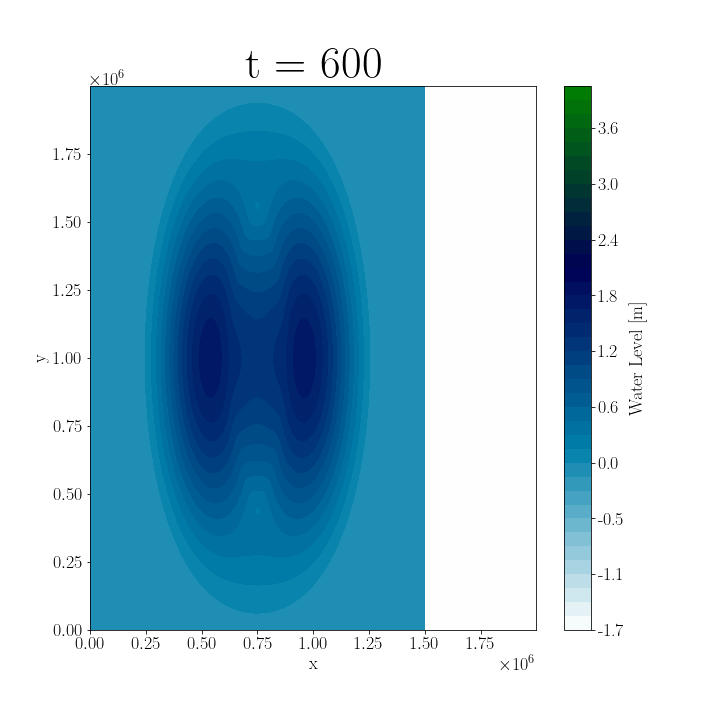
\includegraphics[width=\linewidth]{Figures/5-2.png}
\caption{}
\end{subfigure}

\begin{subfigure}[b]{.4\linewidth}
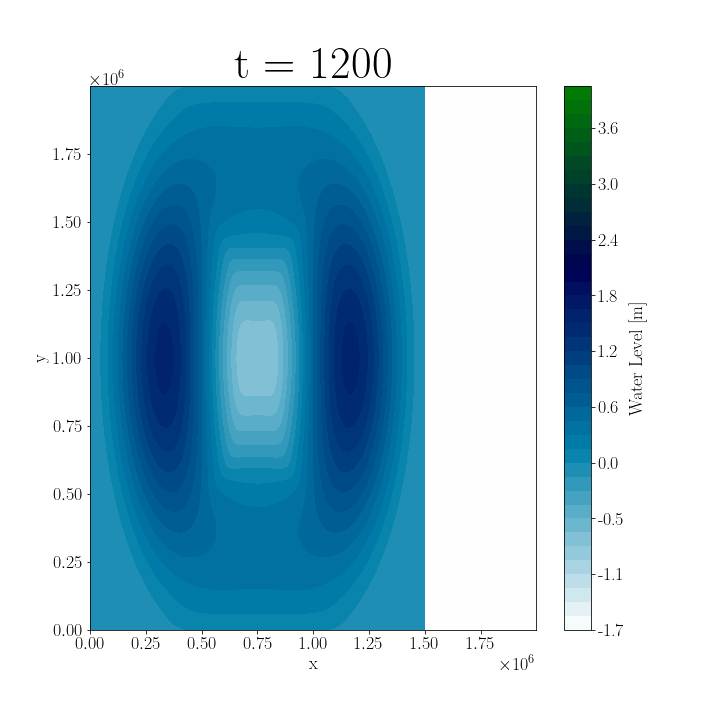
\includegraphics[width=\linewidth]{Figures/5-3.png}
\caption{}
\end{subfigure}
\begin{subfigure}[b]{.4\linewidth}
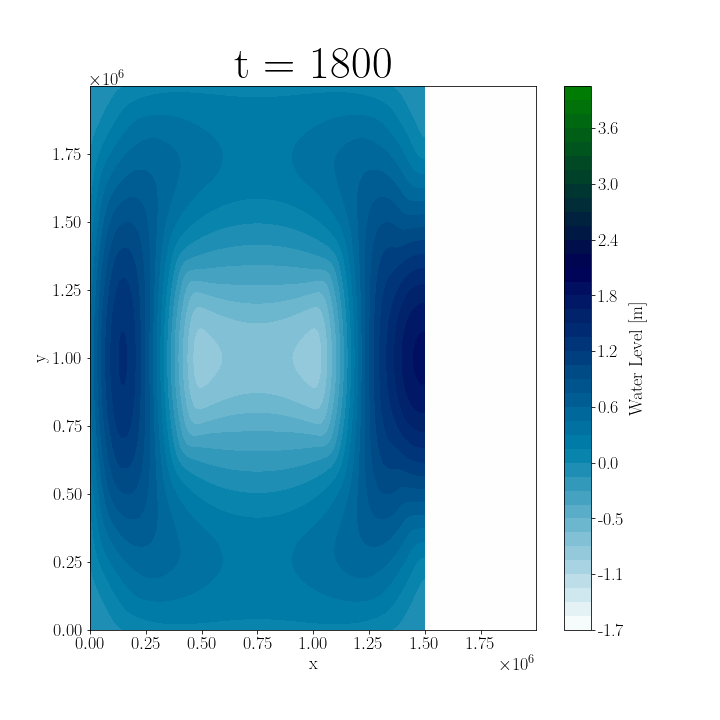
\includegraphics[width=\linewidth]{Figures/5-4.png}
\caption{}
\end{subfigure}

\begin{subfigure}[b]{.4\linewidth}
\includegraphics[width=\linewidth]{Figures/5-5.png}
\caption{}
\end{subfigure}
\begin{subfigure}[b]{.4\linewidth}
\includegraphics[width=\linewidth]{Figures/5-6.png}
\caption{}
\end{subfigure}
\caption{Niveles de agua de la salida de ejecutar el código de LBM optimizado con el archivo de entrada \textbf{Test40000}.}
\label{fig:24}
\end{figure}

%--------------------------------------------

\begin{figure}[H]
\centering
\begin{subfigure}[b]{.4\linewidth}
\includegraphics[width=\linewidth]{Figures/Plots/Antofa1.png}
\caption{desnivel máximo = 4.99 [m]}
\end{subfigure}
\begin{subfigure}[b]{.4\linewidth}
\includegraphics[width=\linewidth]{Figures/Plots/Antofa2.png}
\caption{desnivel máximo = 1.56 [m]}
\end{subfigure}

\begin{subfigure}[b]{.4\linewidth}
\includegraphics[width=\linewidth]{Figures/Plots/Antofa3.png}
\caption{desnivel máximo = 1.08 [m]}
\end{subfigure}
\begin{subfigure}[b]{.4\linewidth}
\includegraphics[width=\linewidth]{Figures/Plots/Antofa4.png}
\caption{desnivel máximo = 0.90 [m]}
\end{subfigure}

\begin{subfigure}[b]{.4\linewidth}
\includegraphics[width=\linewidth]{Figures/Plots/Antofa5.png}
\caption{desnivel máximo = 1.37 [m]}
\end{subfigure}
\begin{subfigure}[b]{.4\linewidth}
\includegraphics[width=\linewidth]{Figures/Plots/Antofa6.png}
\caption{desnivel máximo = 1.38 [m]}
\end{subfigure}
\caption{Niveles de agua de la salida de ejecutar el código de LBM optimizado con el archivo de entrada \textbf{Antofagasta}.}
\label{fig:25}
\end{figure}

%--------------------------------------------

\begin{figure}[H]
\centering
\begin{subfigure}[b]{.4\linewidth}
\includegraphics[width=\linewidth]{Figures/Plots/Serena1.png}
\caption{desnivel máximo = 4.99 [m]}
\end{subfigure}
\begin{subfigure}[b]{.4\linewidth}
\includegraphics[width=\linewidth]{Figures/Plots/Serena2.png}
\caption{desnivel máximo = 0.83 [m]}
\end{subfigure}

\begin{subfigure}[b]{.4\linewidth}
\includegraphics[width=\linewidth]{Figures/Plots/Serena3.png}
\caption{desnivel máximo = 0.71 [m]}
\end{subfigure}
\begin{subfigure}[b]{.4\linewidth}
\includegraphics[width=\linewidth]{Figures/Plots/Serena4.png}
\caption{desnivel máximo = 1.17 [m]}
\end{subfigure}

\begin{subfigure}[b]{.4\linewidth}
\includegraphics[width=\linewidth]{Figures/Plots/Serena5.png}
\caption{desnivel máximo = 0.70 [m]}
\end{subfigure}
\begin{subfigure}[b]{.4\linewidth}
\includegraphics[width=\linewidth]{Figures/Plots/Serena6.png}
\caption{desnivel máximo = 0.50 [m]}
\end{subfigure}
\caption{Niveles de agua de la salida de ejecutar el código de LBM optimizado con el archivo de entrada \textbf{Serena}.}
\label{fig:26}
\end{figure}

%--------------------------------------------

\begin{figure}[H]
\centering
\begin{subfigure}[b]{.4\linewidth}
\includegraphics[width=\linewidth]{Figures/Plots/Valpo1.png}
\caption{desnivel máximo = 4.99 [m]}
\end{subfigure}
\begin{subfigure}[b]{.4\linewidth}
\includegraphics[width=\linewidth]{Figures/Plots/Valpo2.png}
\caption{altura máxima = 501.3 [m]}
\end{subfigure}

\begin{subfigure}[b]{.4\linewidth}
\includegraphics[width=\linewidth]{Figures/Plots/Valpo3.png}
\caption{desnivel máximo = 0.98 [m]}
\end{subfigure}
\begin{subfigure}[b]{.4\linewidth}
\includegraphics[width=\linewidth]{Figures/Plots/Valpo4.png}
\caption{desnivel máximo = 0.77 [m]}
\end{subfigure}

\begin{subfigure}[b]{.4\linewidth}
\includegraphics[width=\linewidth]{Figures/Plots/Valpo5.png}
\caption{desnivel máximo = 1.47 [m]}
\end{subfigure}
\begin{subfigure}[b]{.4\linewidth}
\includegraphics[width=\linewidth]{Figures/Plots/Valpo6.png}
\caption{desnivel máximo = 0.78 [m]}
\end{subfigure}
\caption{Niveles de agua de la salida de ejecutar el código de LBM optimizado con el archivo de entrada \textbf{Valparaiso}.}
\label{fig:27}
\end{figure}
\newpage
\secnumbersection{Conclusiones}
\hlabel{sec:5}

Durante el desarrollo de la presente memoria, se ha podido desarrollar a través del entorno AMD ROCm una versión compilable y ejecutable de un código en base al método de Lattice Boltzmann, que cumple condiciones de borde abierta y resuelve las ecuaciones de agua poco profunda.
Esto se pudo lograr partiendo por una serie de experimentación gradual, necesaria al momento de inicializarse en este tipo de plataformas de desarrollo y programación paralela en general.
Partiendo por problemas como la suma de vectores, multiplicación de matrices y terminando en la implementación del método de Lattice Boltzmann como tal se pudo generar una comparación empírica del uso de los lenguajes HIP y CUDA C en las tarjetas AMD RX570 y NVIDIA GTX960M, ambas de gama media-alta respecto a sus años de lanzamiento.

A partir de los resultados obtenidos, se pudo observar que estos en general presentaron patrones similares en ambas GPUs, tomando en consideración las especificaciones técnicas dadas a conocer en el Capítulo~\hyperref[sec:3.1]{3.1}.
De igual manera, se plantea como esto está justificado por la existencia de la herramienta \textit{Hipify}, la cual tiene una gran importancia a la hora de transformar código de CUDA C a HIP y por tanto, al derribar las limitaciones de la programación de propósito general en GPU, independiente del hardware a disposición.
Este hecho se basa en que, si bien la plataforma ROCm se consolido como tal el año 2015, recién en los últimos años esta ganando una comunidad que permita su desarrollo al publico general, permitiendo su aplicación en investigaciones de \textit{High Performance Computing} como aquellas revisadas en el Capítulo~\hyperref[sec:2]{2}.

Por otro lado, a pesar de los positivos resultados de la puesta en practica de las herramientas y APIs de ROCm, uno de los contras presentes es el dominio limitado de tarjetas gráficas que soportan su uso, conformado por aquellas con chips de generación GFX7, GFX8, CDNA y GFX9 \cite{supportGPU}, además de otras características especificas de la comunicación con el resto de los componentes de la computadora usada.
%Además, se espera que lo anterior junto a la gran demanda de tarjetas gráficas debido a los distintos factores desencadenados por las condiciones actuales no permita el desarrollo de proyectos de GPGPU en ROCm por los siguientes años, al menos a nivel de computadoras personales.

En conclusión, gracias a ROCm se logró para esta memoria ejecuciones del método de Lattice Boltzmann con condiciones de borde abiertas en tarjetas AMD sin precedentes, las cuales sirven como argumentos para afirmar que dicha plataforma tiene potencial para ampliar enormemente el dominio de uso de GPUs en programación paralela en términos de investigación.
%lo cual se podrá lograr en un futuro con las condiciones globales adecuadas y una mayor madurez de la misma. 


\secnumberlesssection{ANEXOS}
\hlabel{sec:6}

\section{Instalación de ROCm y HIP}

A lo largo de la realización de esta memoria, un evento clave fue la instalación de la plataforma principal de desarrollo en HPC, ROCm. 
En el siguiente anexo, se presentará una descripción detallada de los pasos seguidos por el autor para realizar este proceso. 
La mayoría de la información respecto a la instalación fue obtenida de la documentación oficial de ROCm.

\subsection*{Computadores con GPU de AMD y Ubuntu 20.04}

En computadores que poseen una tarjeta gráfica de la marca AMD, el proceso es más simple, pues los paquetes de instalación se encuentran en los gestores de paquetes del repositorio. Los pasos son los siguientes:

\begin{enumerate}
\item Identificar si se tienen instalado el \textit{driver} de AMD para la tarjeta gráfica instalada. 
El output debería ser la información sobre el paquete \textit{amdgpu-pro}.
\begin{lstlisting}[language=bash]
$apt show amdgpu-pro
\end{lstlisting}
\item (Opcional) Instalar el \textit{driver} en caso de ser necesario.
\begin{lstlisting}[language=bash]
$sudo apt install amdgpu-pro
\end{lstlisting}

\item Verificar los grupos del sistema.
\begin{lstlisting}[language=bash]
$groups
\end{lstlisting}

\item Agregar el usuario de trabajo a los grupos \textit{video} y \textit{render}.
En los siguientes comandos \$LOGNAME corresponde al nombre del usuario actual.
\begin{lstlisting}[language=bash]
$sudo usermod -a -G video $LOGNAME
$sudo usermod -a -G render $LOGNAME
\end{lstlisting}

\item Verificar las actualizaciones del sistema.
\begin{lstlisting}[language=bash]
$sudo apt update
$sudo apt dist-upgrade
$sudo apt install libnuma-dev
$sudo reboot
\end{lstlisting}
\item Agregar el repositorio de ROCm al gestor de paquetes.
\begin{lstlisting}[language=bash, breaklines=true]
$sudo apt install wget gpupg2
$wget -q -O - https://repo.radeon.com/rocm/rocm.gpg.key | sudo apt-key add -
$echo 'deb [arch=amd64] https://repo.radeon.com/rocm/apt/debian/ xenial main' | sudo tee /etc/apt/sources.list.d/rocm.list
\end{lstlisting}


\item Instalar dependencias previas.
\begin{lstlisting}[language=bash]
$sudo apt install mesa-common-dev
$sudo apt install clang
$sudo apt install comgr
\end{lstlisting}

\item Instalar ROCm y reiniciar el sistema.
\begin{lstlisting}[language=bash]
$sudo apt update
$sudo apt install rocm-dkms && sudo reboot
\end{lstlisting}
\item Revisar si ROCm se instaló correctamente ejecutando los siguientes comandos.
El output debería ser el nombre del modelo de la GPU en el sistema.
\begin{lstlisting}[language=bash]
$/opt/rocm/bin/rocminfo
$/opt/rocm/opencl/bin/clinfo
\end{lstlisting}

\item Revisar si HIP se instaló correctamente ejecutando el siguiente comando. 
El output debería ser información sobre la plataforma en general (compilador utilizado, tarjeta gráfica de la plataforma, etc.).

\begin{lstlisting}[language=bash]
$/opt/rocm/bin/hipconfig --full
\end{lstlisting}

\item Agregar a la variable de entorno \textit{PATH} el directorio de instalación de ROCm. Esto se hace editando el archivo \textasciitilde/.bashrc y anexando la siguiente linea al final.
\begin{lstlisting}[language=bash, breaklines=true]
export PATH=$PATH:/opt/rocm/bin:/opt/rocm/rocprofiler/bin:/opt/rocm/opencl/bin
\end{lstlisting}
\end{enumerate}

\subsection*{Computadores con GPU de NVIDIA y Ubuntu 20.04}

En computadores que poseen una tarjeta gráfica de la marca NVIDIA, el proceso es un poco más complejo, pues el paquete de instalación de \textit{hip-nvcc} (compilador que utiliza \textit{nvcc} como base de la plataforma) no se encuentra actualmente disponible por errores de dependencia entre las versiones actuales de CUDA. Se asume que el equipo en el cual se trabajará ya tiene un paquete de CUDA SDK instalado en el sistema.

\begin{enumerate}
\item Instalar la plataforma base de ROCm, haciendo uso de los puntos 3, 4, 5, 6,7, 8 y 11 de la sección anterior.

\item Instalar cmake en caso de no tenerlo.

\begin{lstlisting}[language=bash]
$sudo apt install cmake
\end{lstlisting}

\item Instalar ROCclr.
Como prerrequisito, ROCclr necesita \textit{mesa-common-dev}, \textit{comgr}, \textit{clang} y \textit{ROCm Device Library}.
Los 3 primeros paquetes pueden ser instalados utilizando un gestor de paquetes, sin embargo, a continuación se dejarán enlaces a los respectivos github para la construcción detallada de aquellos paquetes que pueden instalarse manualmente.
\begin{itemize}
    \item COMGR: \hyperlink{https://github.com/RadeonOpenCompute/ROCm-CompilerSupport}{https://github.com/RadeonOpenCompute/ROCm-CompilerSupport}
    \item CLang: \hyperlink{https://github.com/RadeonOpenCompute/llvm-project}{https://github.com/RadeonOpenCompute/llvm-project}
    \item ROCm Device Library: \hyperlink{https://github.com/RadeonOpenCompute/ROCm-Device-Libs}{https://github.com/RadeonOpenCompute/ROCm-Device-Libs}
\end{itemize}
\begin{lstlisting}[language=bash, breaklines=true]
$git clone -b rocm-4.2.x https://github.com/ROCm-Developer-Tools/ROCclr.git
$export ROCclr_DIR="$(readlink -f ROCclr)"
$git clone -b rocm-4.2.x https://github.com/RadeonOpenCompute/ROCm-OpenCL-Runtime.git
$export OPENCL_DIR="$(readlink -f ROCm-OpenCL-Runtime)"
$cd "$ROCclr_DIR"
$mkdir -p build;cd build
$cmake -DOPENCL_DIR="$OPENCL_DIR" -DCMAKE_INSTALL_PREFIX=/opt/rocm/rocclr ..
$make -j
$sudo make install
\end{lstlisting}
\item Instalar HIP.
\begin{lstlisting}[language=bash, breaklines=true]
$export HIP_DIR="$(readlink -f HIP)"
$cd "$HIP_DIR"
$mkdir -p build; cd build
$cmake -DCMAKE_PREFIX_PATH="$ROCclr_DIR/build;/opt/rocm/" -DCMAKE_INSTALL_PREFIX=</where/to/install/hip> ..
$make -j
$sudo make install
\end{lstlisting}

\item Verificar la integridad de HIP ejecutando el siguiente comando. Los atributos \textit{platform} y \textit{compiler} deberían ser \textit{nvidia} y \textit{nvcc} respectivamente.

\begin{lstlisting}[language=bash]
$/opt/rocm/bin/hipconfig --full
\end{lstlisting}

\item Modificar la variable de entorno CUDA\_PATH en caso de que el punto anterior no se cumpla, igualándola al directorio de instalación de CUDA.
\end{enumerate}

Para mayor información, referirse a la documentación oficial de AMD ROCm.
\begin{itemize}
    \item \hyperlink{https://rocmdocs.amd.com/en/latest/Installation_Guide/Installation-Guide.html}{https://rocmdocs.amd.com/en/latest/Installation\_Guide/Installation-Guide.html}
    \item \hyperlink{https://rocmdocs.amd.com/en/latest/Installation_Guide/HIP-Installation.html}{https://rocmdocs.amd.com/en/latest/Installation\_Guide/HIP-Installation.html}
\end{itemize}

\newpage

\section{Métodos de HIP que dan soporte a métodos de CUDA C}

En el detalle de la experimentación realizada, se explica como ROCm a través de su lenguaje de programación HIP presenta soporte a gran parte de las APIs ofrecidas por el lenguaje CUDA C \cite{support}, las mismas que generan un cambio en los archivos de entrada al momento de utilizar la herramienta \textit{Hipify}. 

En la siguiente tabla se plantea una selección de los principales métodos presentes en los códigos analizados y que a su vez son imprescindibles a la hora de realizar GPGPU tanto en ROCm como en CUDA.

\begin{table}[h!]
\footnotesize
\begin{tabularx}{\textwidth}{|p{0.23\textwidth}|p{0.23\textwidth}|X|}
\hline
API de ROCm           & API de CUDA            & Descripción                                                                                                                                                                                                                   \\ \hline
hipLaunchKernelGGL    & $<<>>$                 & Ejecuta un kernel definido. En ROCm, el método hipLaunchKernelGGL reemplaza a la sintaxis de CUDA $<<>>$, además de incluir un parámetro para la asignación adicional de memoria compartida.                                  \\ \hline
hipMalloc             & cudaMalloc             & Realiza un \textit{Memory Allocation} o asignación de memoria dentro de los registros global de la GPU. Los parámetros de las funciones son un puntero del tipo de dato deseado y el tamaño en bytes a asignar. \\ \hline
hipFree               & cudaFree               & Libera la memoria asignada por hipMalloc/cudaMalloc.                                                                                                                                                                          \\ \hline
hipMemcpy             & cudaMemcpy             & Copia datos en memoria entre CPU y GPU o viceversa.                                                                                                                                                                           \\ \hline
hipFuncSetCacheConfig & cudaFuncSetCacheConfig & Configura el tipo de memoria compartida preferida al momento de ejecutar kernels.                                                                                                                                             \\ \hline
\_\_syncthreads       & \_\_syncthreads        & Genera una barrera a nivel de bloque de \textbackslash{}textit\{threads\}.                                                                                                                                                    \\ \hline
hipGetLastError       & cudaGetLastError       & Obtiene el ultimo error producido en tiempo de ejecución.                                                                                                                                                                     \\ \hline
hipEventCreate        & cudaEventCreate        & A partir de un puntero de tipo hipEvent\_t o cudaEvent\_t retorna un objeto de dicho tipo.                                                                                                                                    \\ \hline
hipEventRecord        & cudaEventRecord        & Captura las condiciones de un flujo de operaciones en un objeto de tipo hipEvent\_t o cudaEvent\_t                                                                                                                            \\ \hline
hipEventSynchronize   & cudaEventSynchronize   & Genera una barrera, la cual espera a que el parámetro de tipo evento se complete para poder continuar con el flujo de instrucciones.                                                                                          \\ \hline
hipEventElapsedTime   & cudaEventElapsedTime   & Retorna el tiempo en milisegundos ocurrido entre dos eventos.                                                                                                                                                                 \\ \hline
\end{tabularx}
\end{table}

\newpage

\section{Repositorios}

\begin{itemize}
    \item LBM\_Framework \href{https://github.com/ASSalinasE/LBM_Framework}{https://github.com/ASSalinasE/LBM\_Framework} en donde se encuentra el framework para CUDA del método de Lattice Boltman, el cual fue modificado para la experimentación del capitulo 5.
    \item LBM-SWE-OBC-CUDA \href{http://www.overleaf.comhttps://github.com/ASSalinasE/LBM-SWE-OBC-CUDA}{https://github.com/ASSalinasE/LBM-SWE-OBC-CUDA}, implementación optimizada en CUDA del método de Lattice Boltmann para resolver las ecuaciones de agua poco profunda con condiciones de borde abiertas.
    \item Memoria-2021 \href{https://github.com/darklambda/Memoria-2021}{https://github.com/darklambda/Memoria-2021}, en donde se pueden encontrar la mayoría de los programas tanto para CUDA como los generados por Hipify-Perl para la experimentación general de la memoria.
\end{itemize}

\section{Uso de herramienta Hipify-Perl y compilador HIPCC}

Durante el trabajo de esta memoria, se utilizó principalmente el software Hipify en su versión en base a Perl para la transformación de programas en CUDA C a HIP para poder ser ejecutados en computadoras con tarjeta de video AMD.
La ejecución de la herramienta consta de, una vez instalada en el sistema, ejecutar el siguiente comando en consola:
\begin{lstlisting}[language=bash, breaklines=true]
$hipify-perl [Input] > [Output]
\end{lstlisting}
en donde Input corresponde a la ruta del archivo de entrada en CUDA C y Output es el nombre del archivo de salida a generar, en el mismo directorio de ejecución del comando.
Si no se declarase un nombre de archivo de salida y se ejecutase el comando tan solo como
\begin{lstlisting}[language=bash, breaklines=true]
$hipify-perl [Input]
\end{lstlisting}
el contenido del archivo de salida se mostraría por pantalla en la consola o terminal.
Una vez realizado lo anterior, debido a que Hipify-Perl es una aplicación directa del análisis gramático de CUDA C, se recomienda revisar los archivos transformados, con tal de encontrar métodos de CUDA pendientes de cambio por algún error en la ejecución.

Finalmente, una vez se tienen todos los archivos preparados, la forma de compilar todo es usar el compilador HIPCC a través del siguiente comando
\begin{lstlisting}[language=bash, breaklines=true]
hipcc -o [Executable] [Source1,Source2,Source3...]
\end{lstlisting}
en donde Executable es el nombre del ejecutable a compilar y SourceX es la dirección relativa de los archivos a partir de los cuales se hará la compilación. 

\newpage
% Bibliografía estilo APA:
%\bibliographystyle{apalike-es}
%\bibliography{bibliografia}{}
\printbibliography

\end{document}
